%!TEX program = xelatex
\documentclass[cn,hazy,pku,12pt,normal,math=newtx,cite=super]{elegantnote}
\title{循环伏安法解析电极极化}

\author{刘松瑞 \quad 2100011819 \\ 组号:24 \quad 组内编号:5}
\institute{化学与分子工程学院}

\expdate{\zhdate{2023/11/2}}
\temperature{22.31 \si{^{\circ}C}}
\pressure{100.39 \si{kPa}}

\usepackage{gensymb}
\usepackage{array}
\usepackage{subfigure}
\usepackage[fontset=windows]{ctex}
\usepackage{graphicx}
\usepackage{float}
\usepackage{caption}
\usepackage{multirow}
%\usepackage{subfig}
%\usepackage{float}
\begin{document}

\maketitle

\keywords{循环伏安法\quad ORR \quad MOR \quad铂电极\quad直接甲醇燃料电池}

\abstracts{

本次实验采用循环伏安法与线性扫描伏安法,对氧气电化学还原反应与甲醇电化学氧化反应
进行测量。通过实验数据分析,扫描速率越快
电流峰值时的电压值近乎不变,而电流峰值升高;搅拌速率升高,传质速率升高,反应速率加快
因此还原电流升高。同时由于浓度分布不均,还原电流会出现振荡现象。进一步可以计算出铂电极的电化学活性面积为 ESA = 2.39 $\rm mm^2$。
通过 ORR 与 MOR 的 CV 曲线可以计算得到甲醇直接燃料电池的极化曲线与输出
功率-输出电压曲线。在甲醇直接燃料电池最大功率时,电压为 0.35 V,
功率为 0.243 $\rm \mu W$。

}

\newpage


\section{引言}

\subsection{实验目的与原理}

实验目的与原理详见预习报告图~\ref{1}。 \cite{pcl2002}

\begin{figure}[htbp]
    \centering
    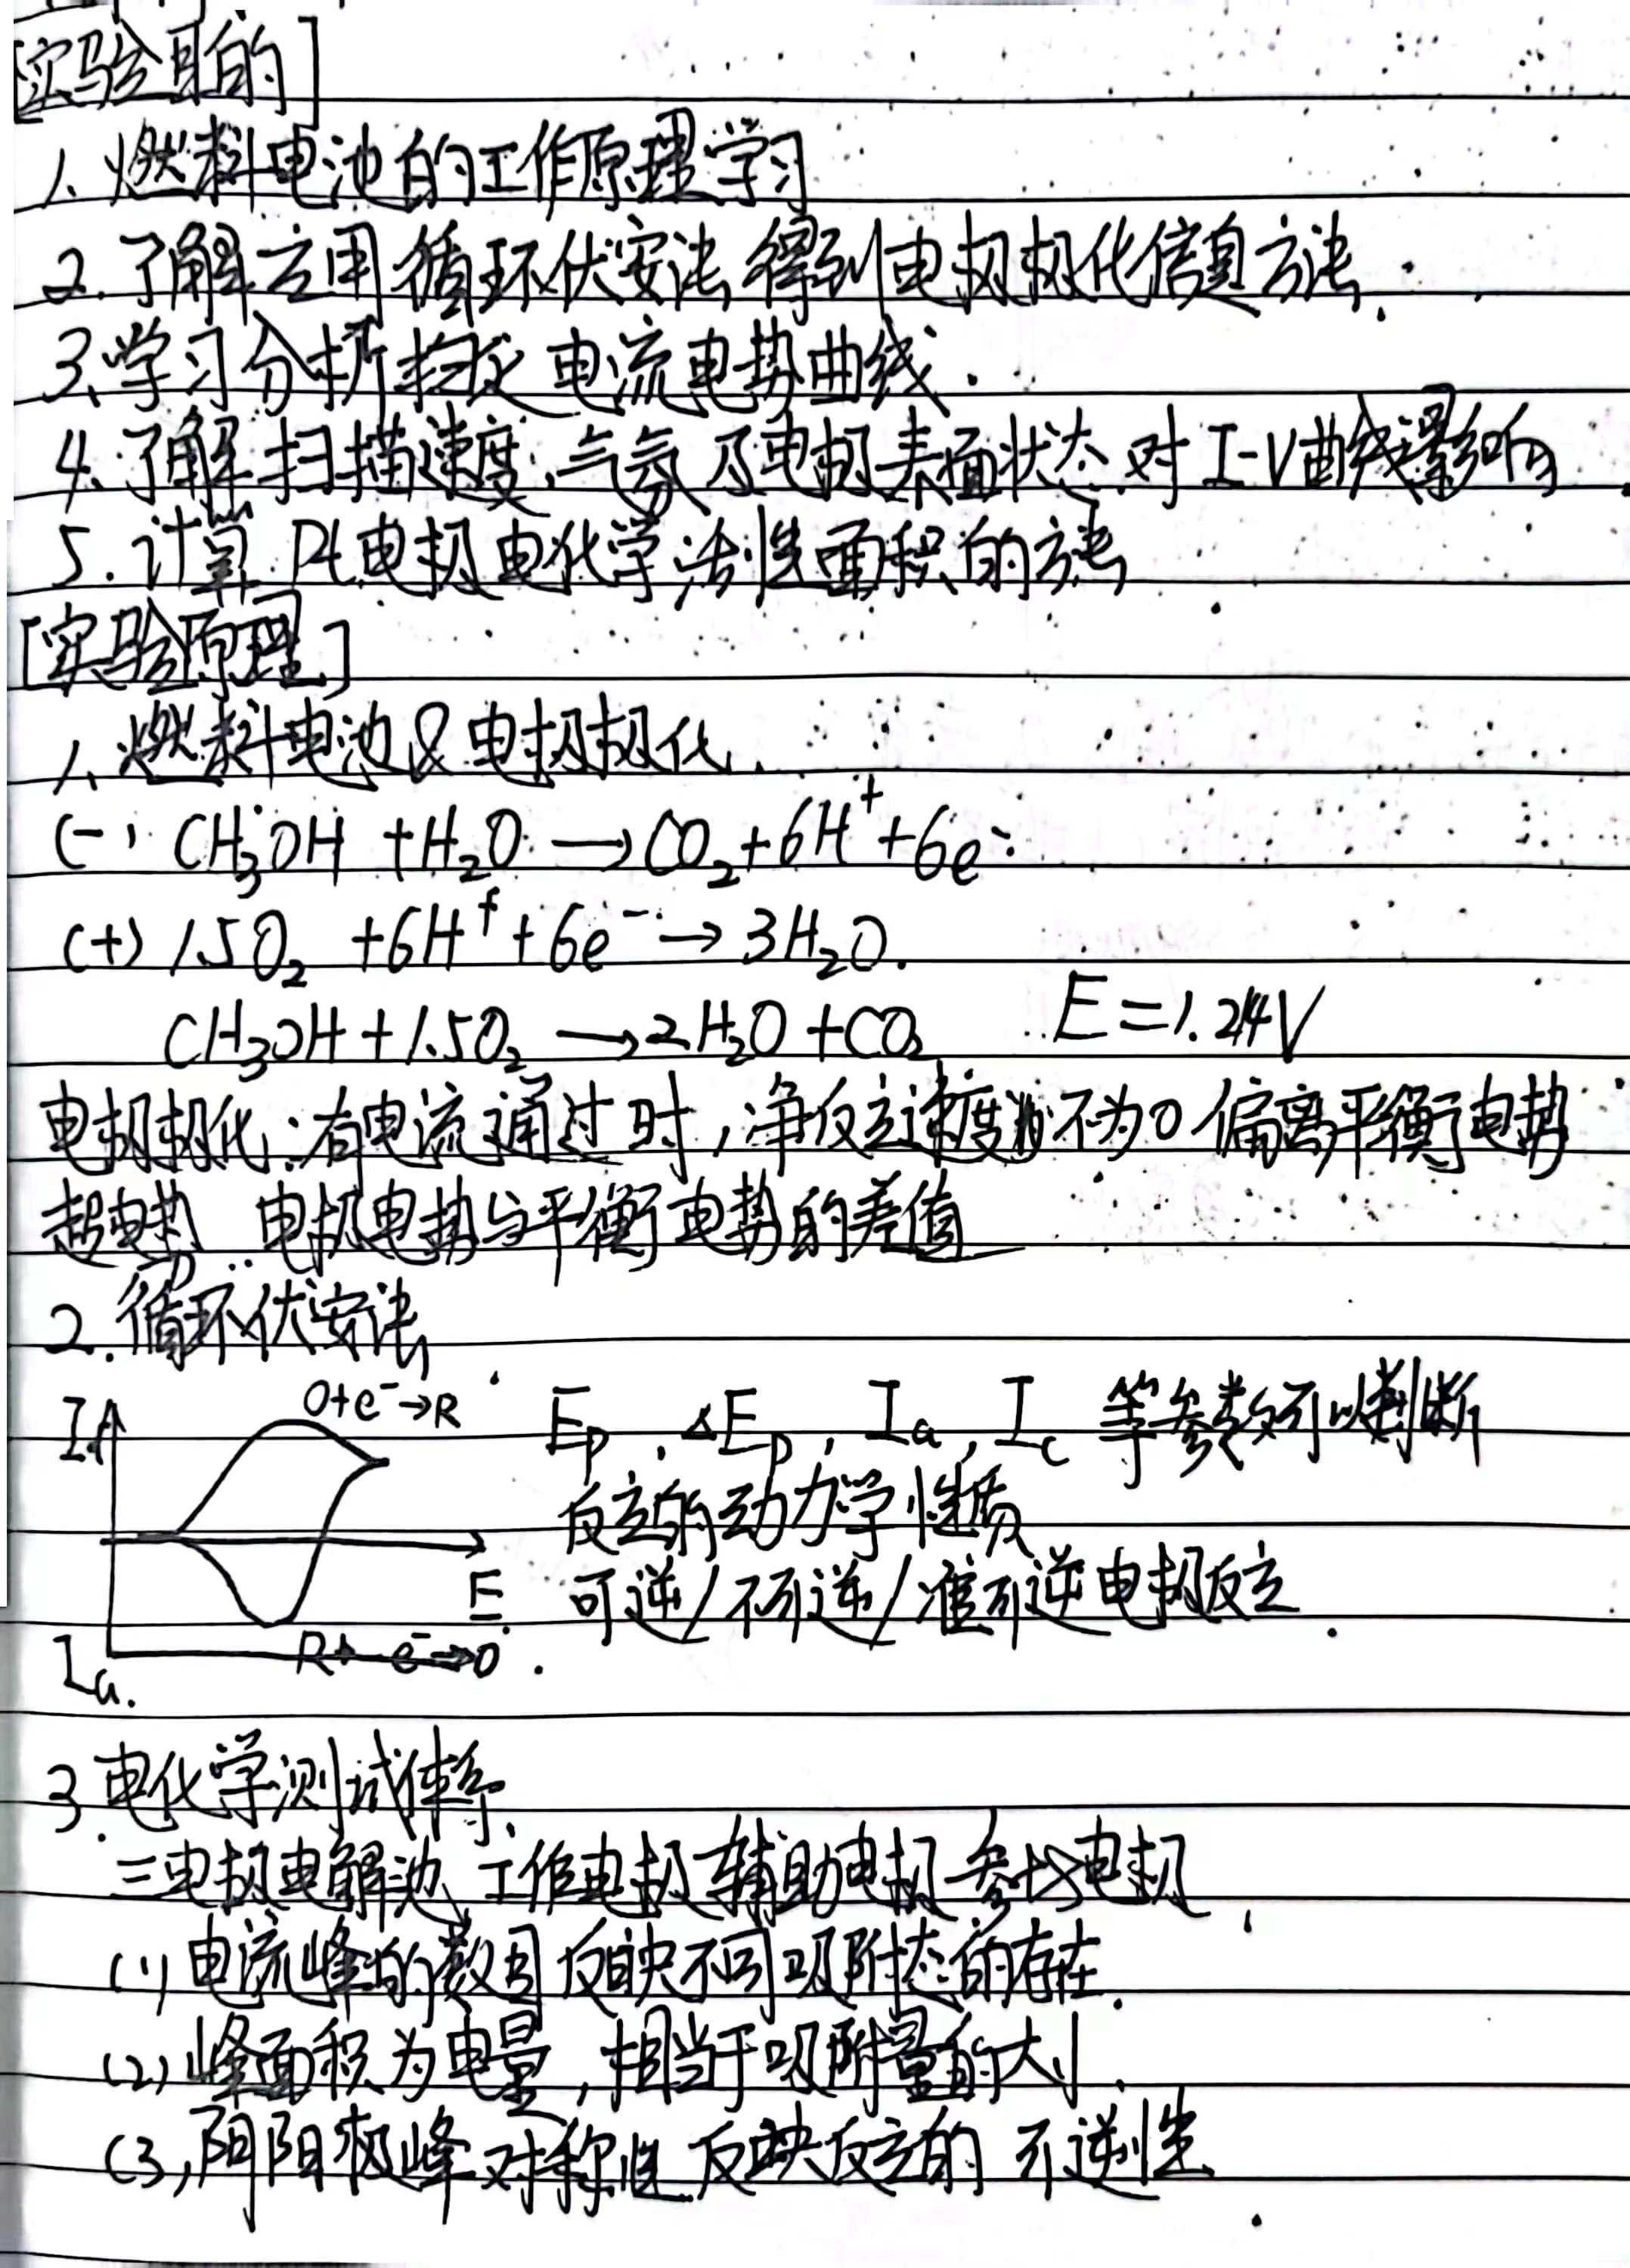
\includegraphics[width = .70\textwidth]{image/yxbg_1.jpg}
    \caption{实验的目的与原理}\label{1}
\end{figure}

\subsection{实验方法}

使用循环伏安法与线性扫描伏安法对铂电极表面的氧还原反应与铂电极表面的甲醇电化学氧化反应进行测定伏安曲线。


\section{实验部分}

\subsection{实验步骤}

实验步骤详见预习报告图~\ref{b} 。
\begin{figure}[htbp]
    \centering
    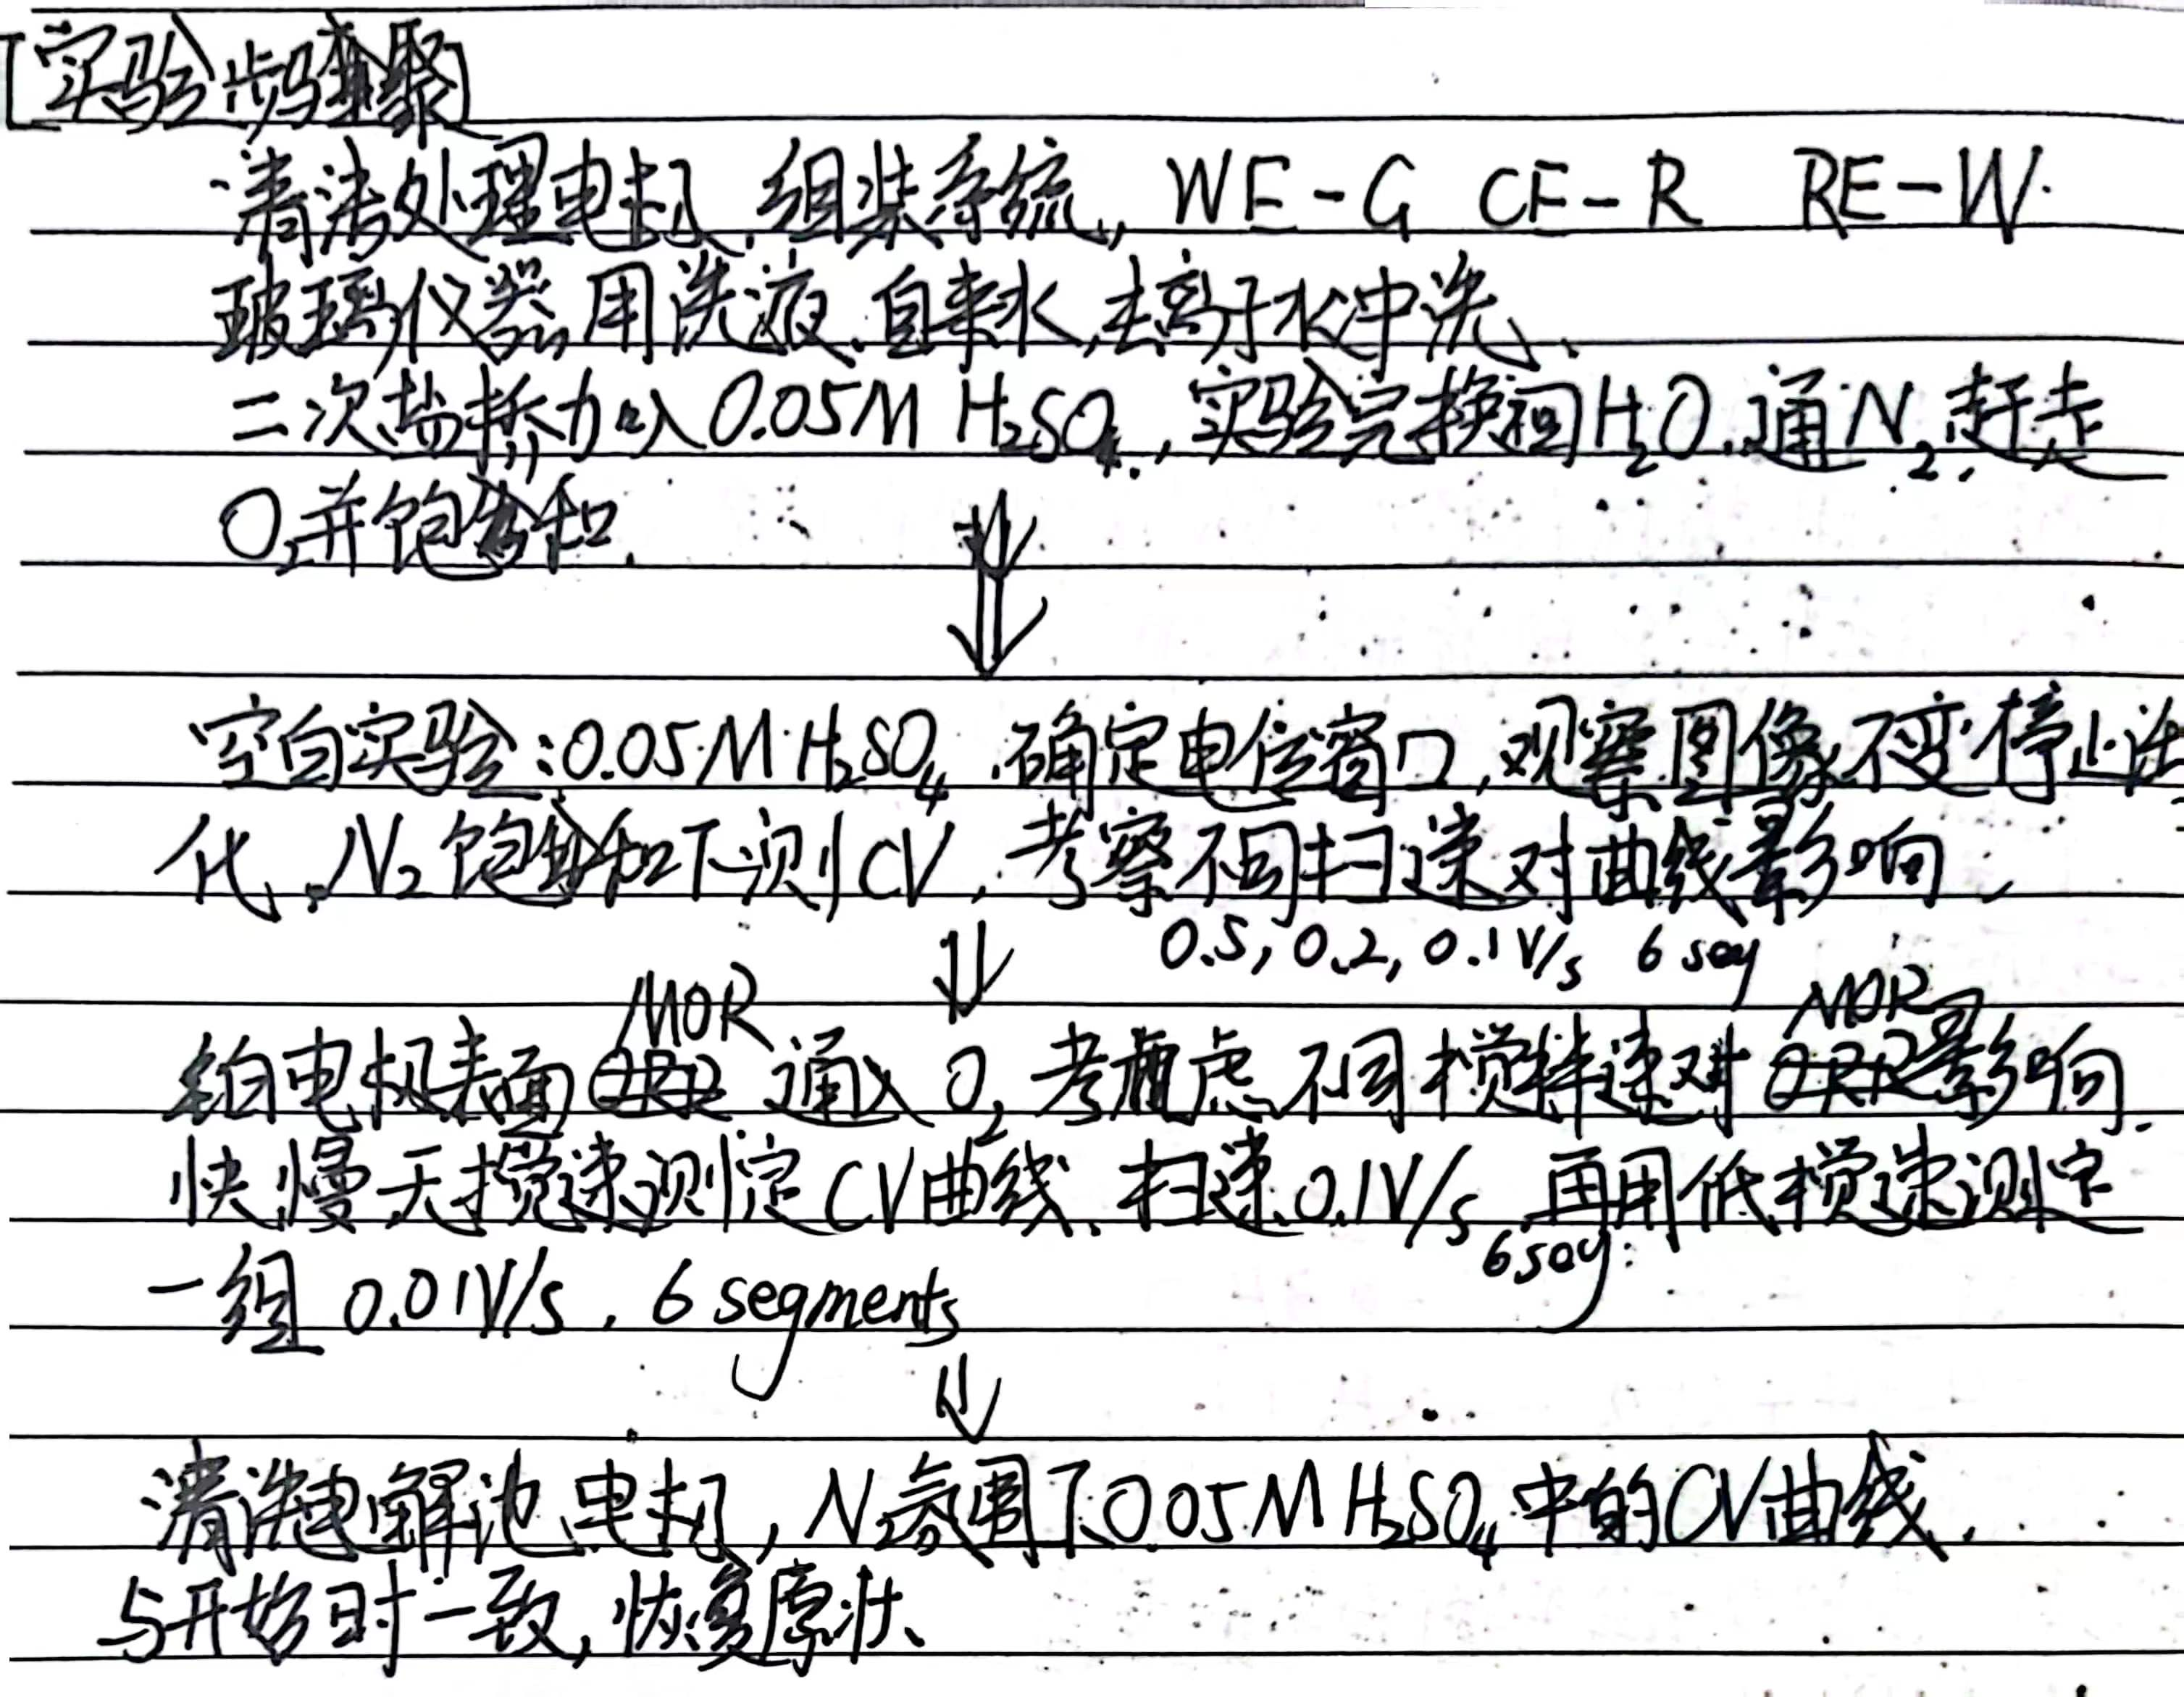
\includegraphics[width = .70\textwidth]{image/yxbg_2.jpg}
    \caption{实验步骤}\label{b}
\end{figure}


\subsection{仪器与药品}

\begin{enumerate} %有序列表
    \item 试剂 \\   0.05 mol/L 硫酸,0.10 mol/L 硫酸,0.10 mol/L 甲醇水溶液。

    \item 仪器 \\   三电极电解池,W.E. 为铂盘电极,C.E. 为铂片电极,R.E. 为双盐桥饱和甘汞电极。
    CHI 电化学工作站,磁力搅拌恒温槽,温度计,氧气钢瓶,氮气钢瓶。
\end{enumerate}

\section{实验现象与数据处理}

本次实验使用参比电极为饱和甘汞电极,辅助电极为铂片电极,工作电极为铂盘电极,下面所描述的电势均为相对于饱和甘汞电极的相对电势,不再在正文中赘述。

\subsection{氮气饱和下测定不同扫速的 CV 曲线}

在 $\rm N_2$ 饱和下,测定不同扫速(0.5 V/s、0.2 V/s、0.1 V/s)的 0.05 mol/L 硫
酸溶液的 CV 曲线,取 Segments 7、8 的数据,如图 \ref{4} 。

\begin{figure}[htbp]
    \centering
    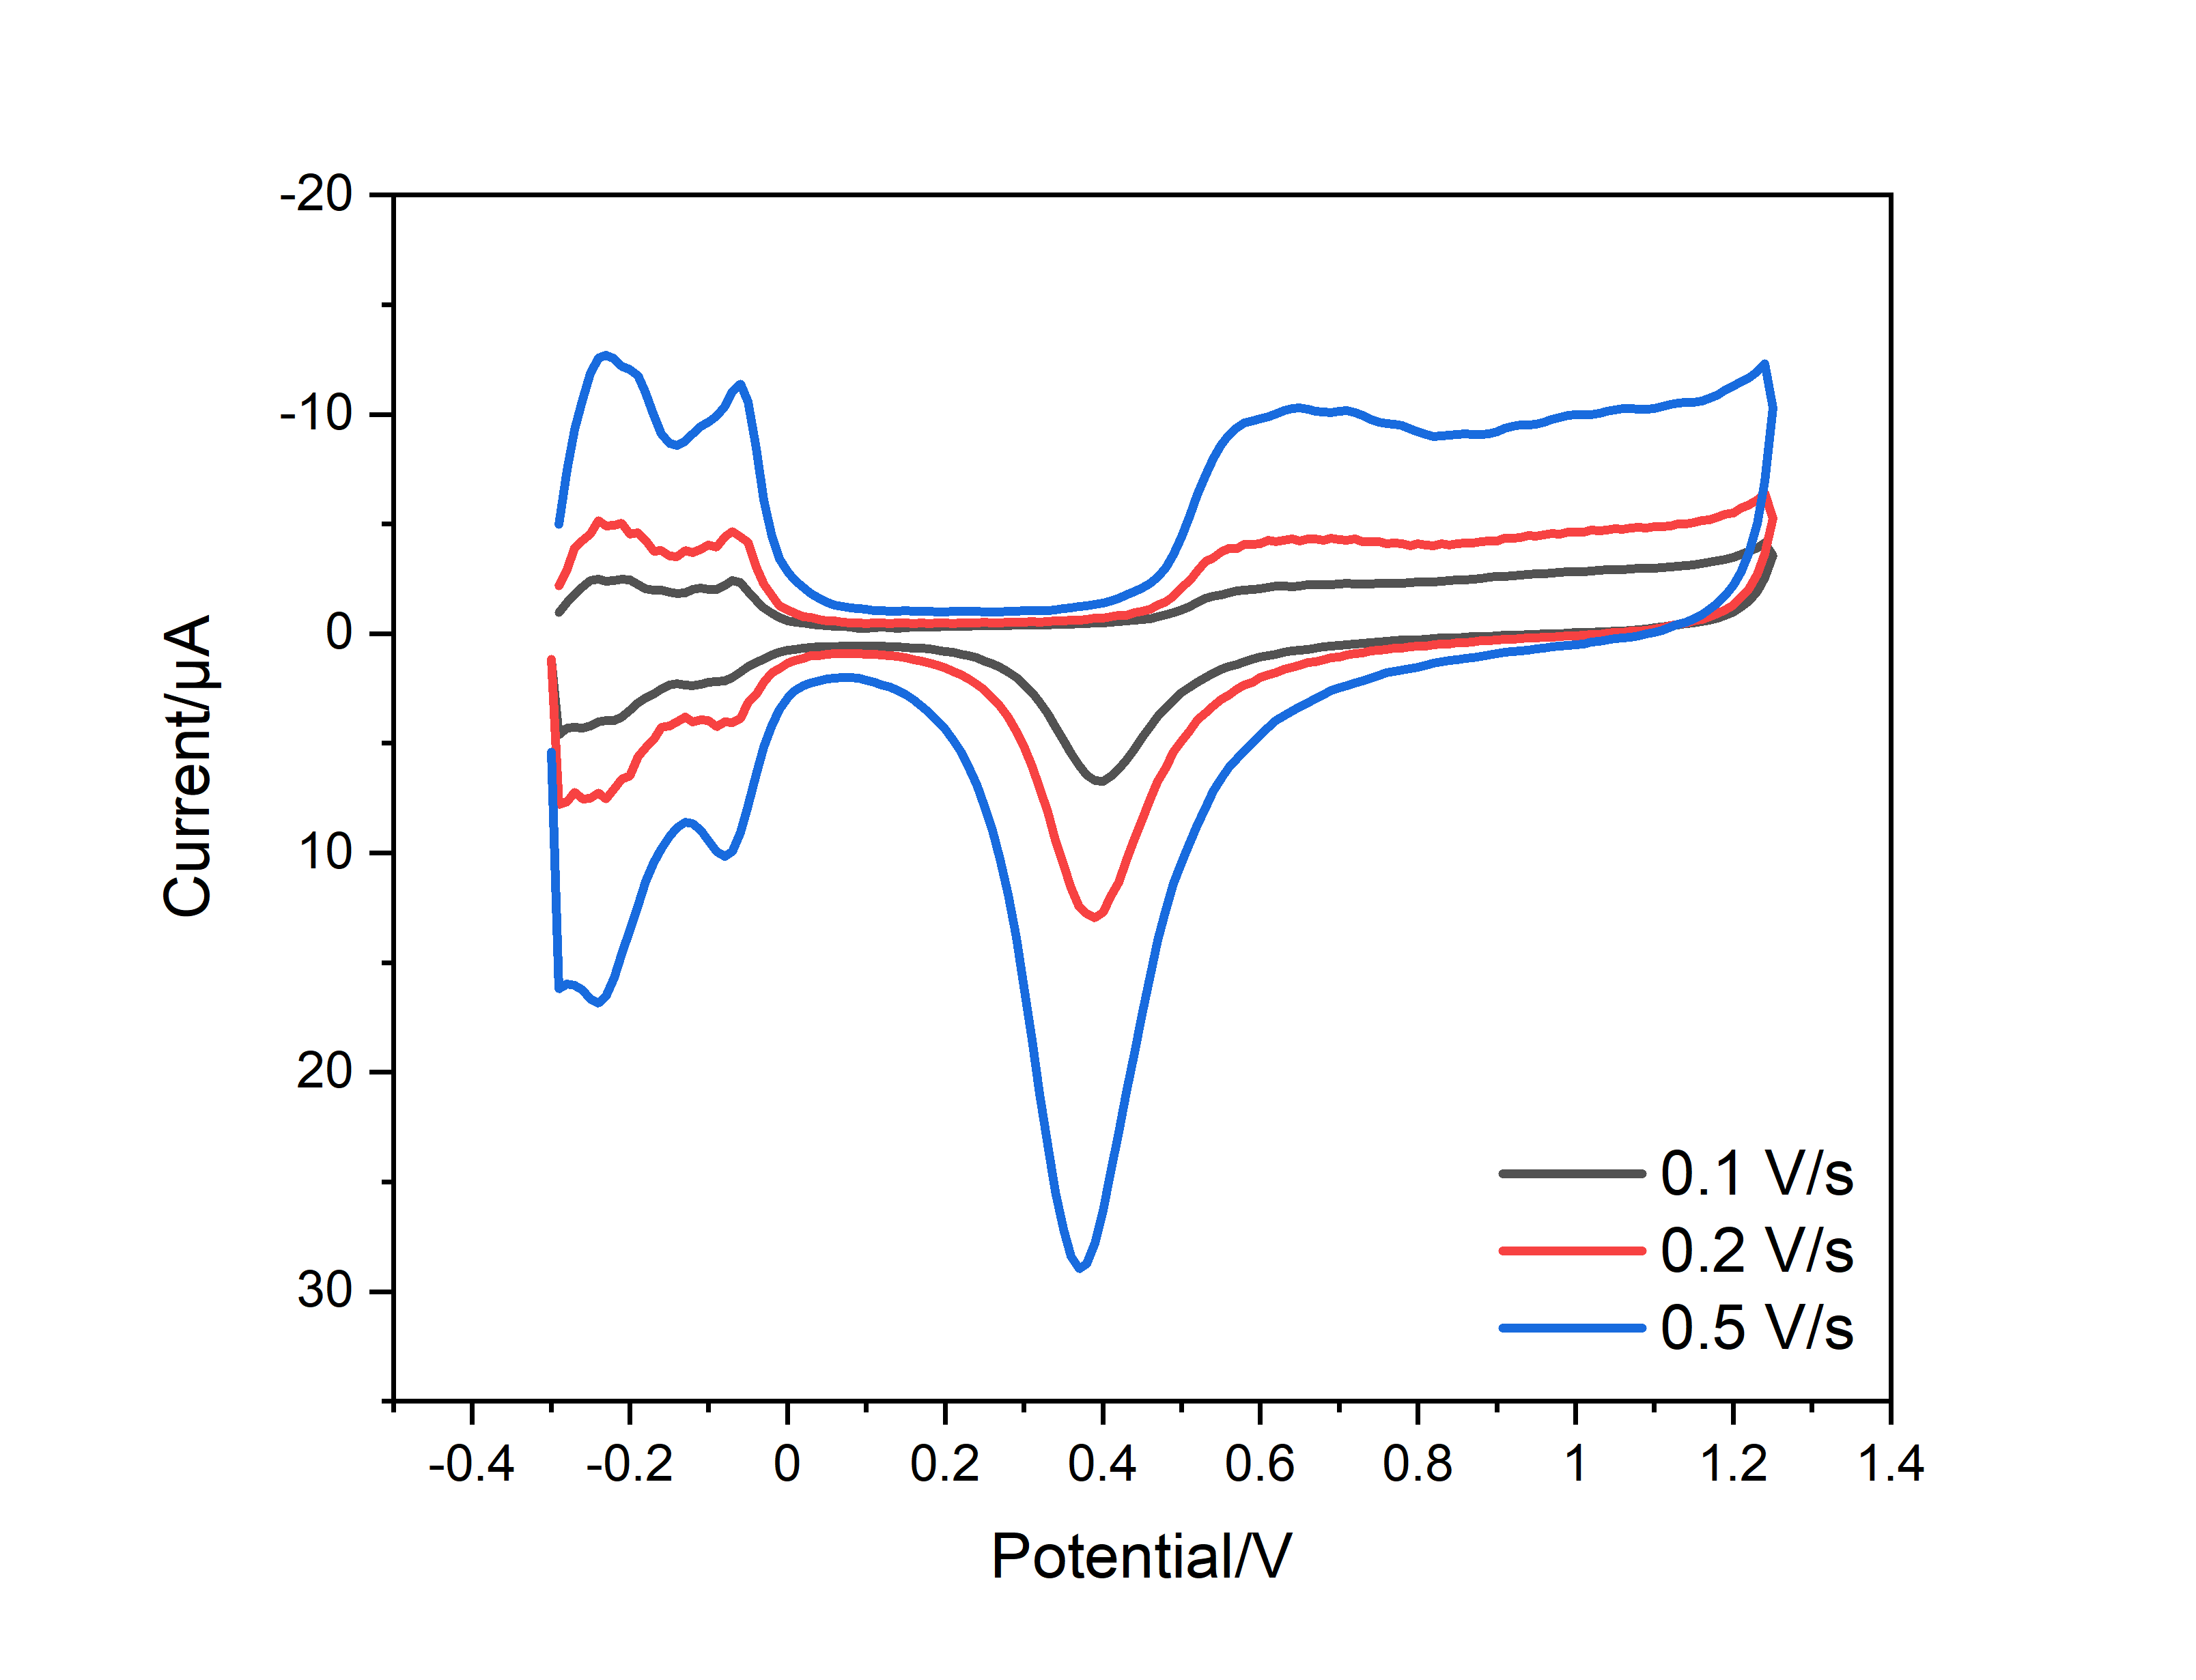
\includegraphics[width = .70\textwidth]{image/Graph7.png}
    \caption{不同扫速 0.05 mol/L 硫酸溶液的 CV 曲线图}\label{4}
\end{figure}

观察图 \ref{4} 可以得出,电流最大处的电势大小与扫速无关,但是电流的峰值大小则与扫速有关,扫速越快峰值越大。
左侧两峰氢区的对称性较好,说明反应的可逆性好,也即氢的吸附-脱附可逆性好;
右侧氧区峰型无对称峰,说明发生了不可逆的还原反应。

\subsection{计算铂电极电化学活性面积}

选取扫速为 0.1 V/s 的氮气饱和下的 CV 曲线来进行计算,对其的氢脱附区积分如图 6 所示。
取双电层的上基线作为积分基线,积分可得:$|S|$ = 0.593 $\rm \mu A \cdot V$,减去双电层的电流可得
$|S|$ =  0.502 $\rm \mu A \cdot V$,则氢的脱附电量为

$$
\rm Q = \int_{}^{} \frac{I}{v} \,dV = \frac{|S|}{v} = \frac{0.502}{0.1} = 5.02\ \mu C 
$$

因此,铂电极的电化学活性面积为

$$
\rm ESA = \frac{Q}{2.10\ \mu C \cdot mm^{-2}} = \frac{5.02\ C}{2.10\ \mu C \cdot mm^{-2}} = 2.39\ mm^{2}
$$



\subsection{氧气饱和下测定不同搅拌速度的 CV 曲线}

在 $\rm O_2$ 饱和下,测定不同搅拌速度的 CV 曲线,扫速为 0.1 V/s,取 Segment 8 的数据,
如图 \ref{5}。并将同扫速下 $\rm O_2$ 与 $\rm N_2$ 饱和的硫酸溶液中铂电极的 CV 曲线还原支进行对比
并求两者的电流差,如图 \ref{6} 与  \ref{7} 。由图  \ref{7} 可得,起始还原电位为 0.590 V。在起始还原电位后
差值明显上升。

\begin{figure}[htbp]
    \centering
    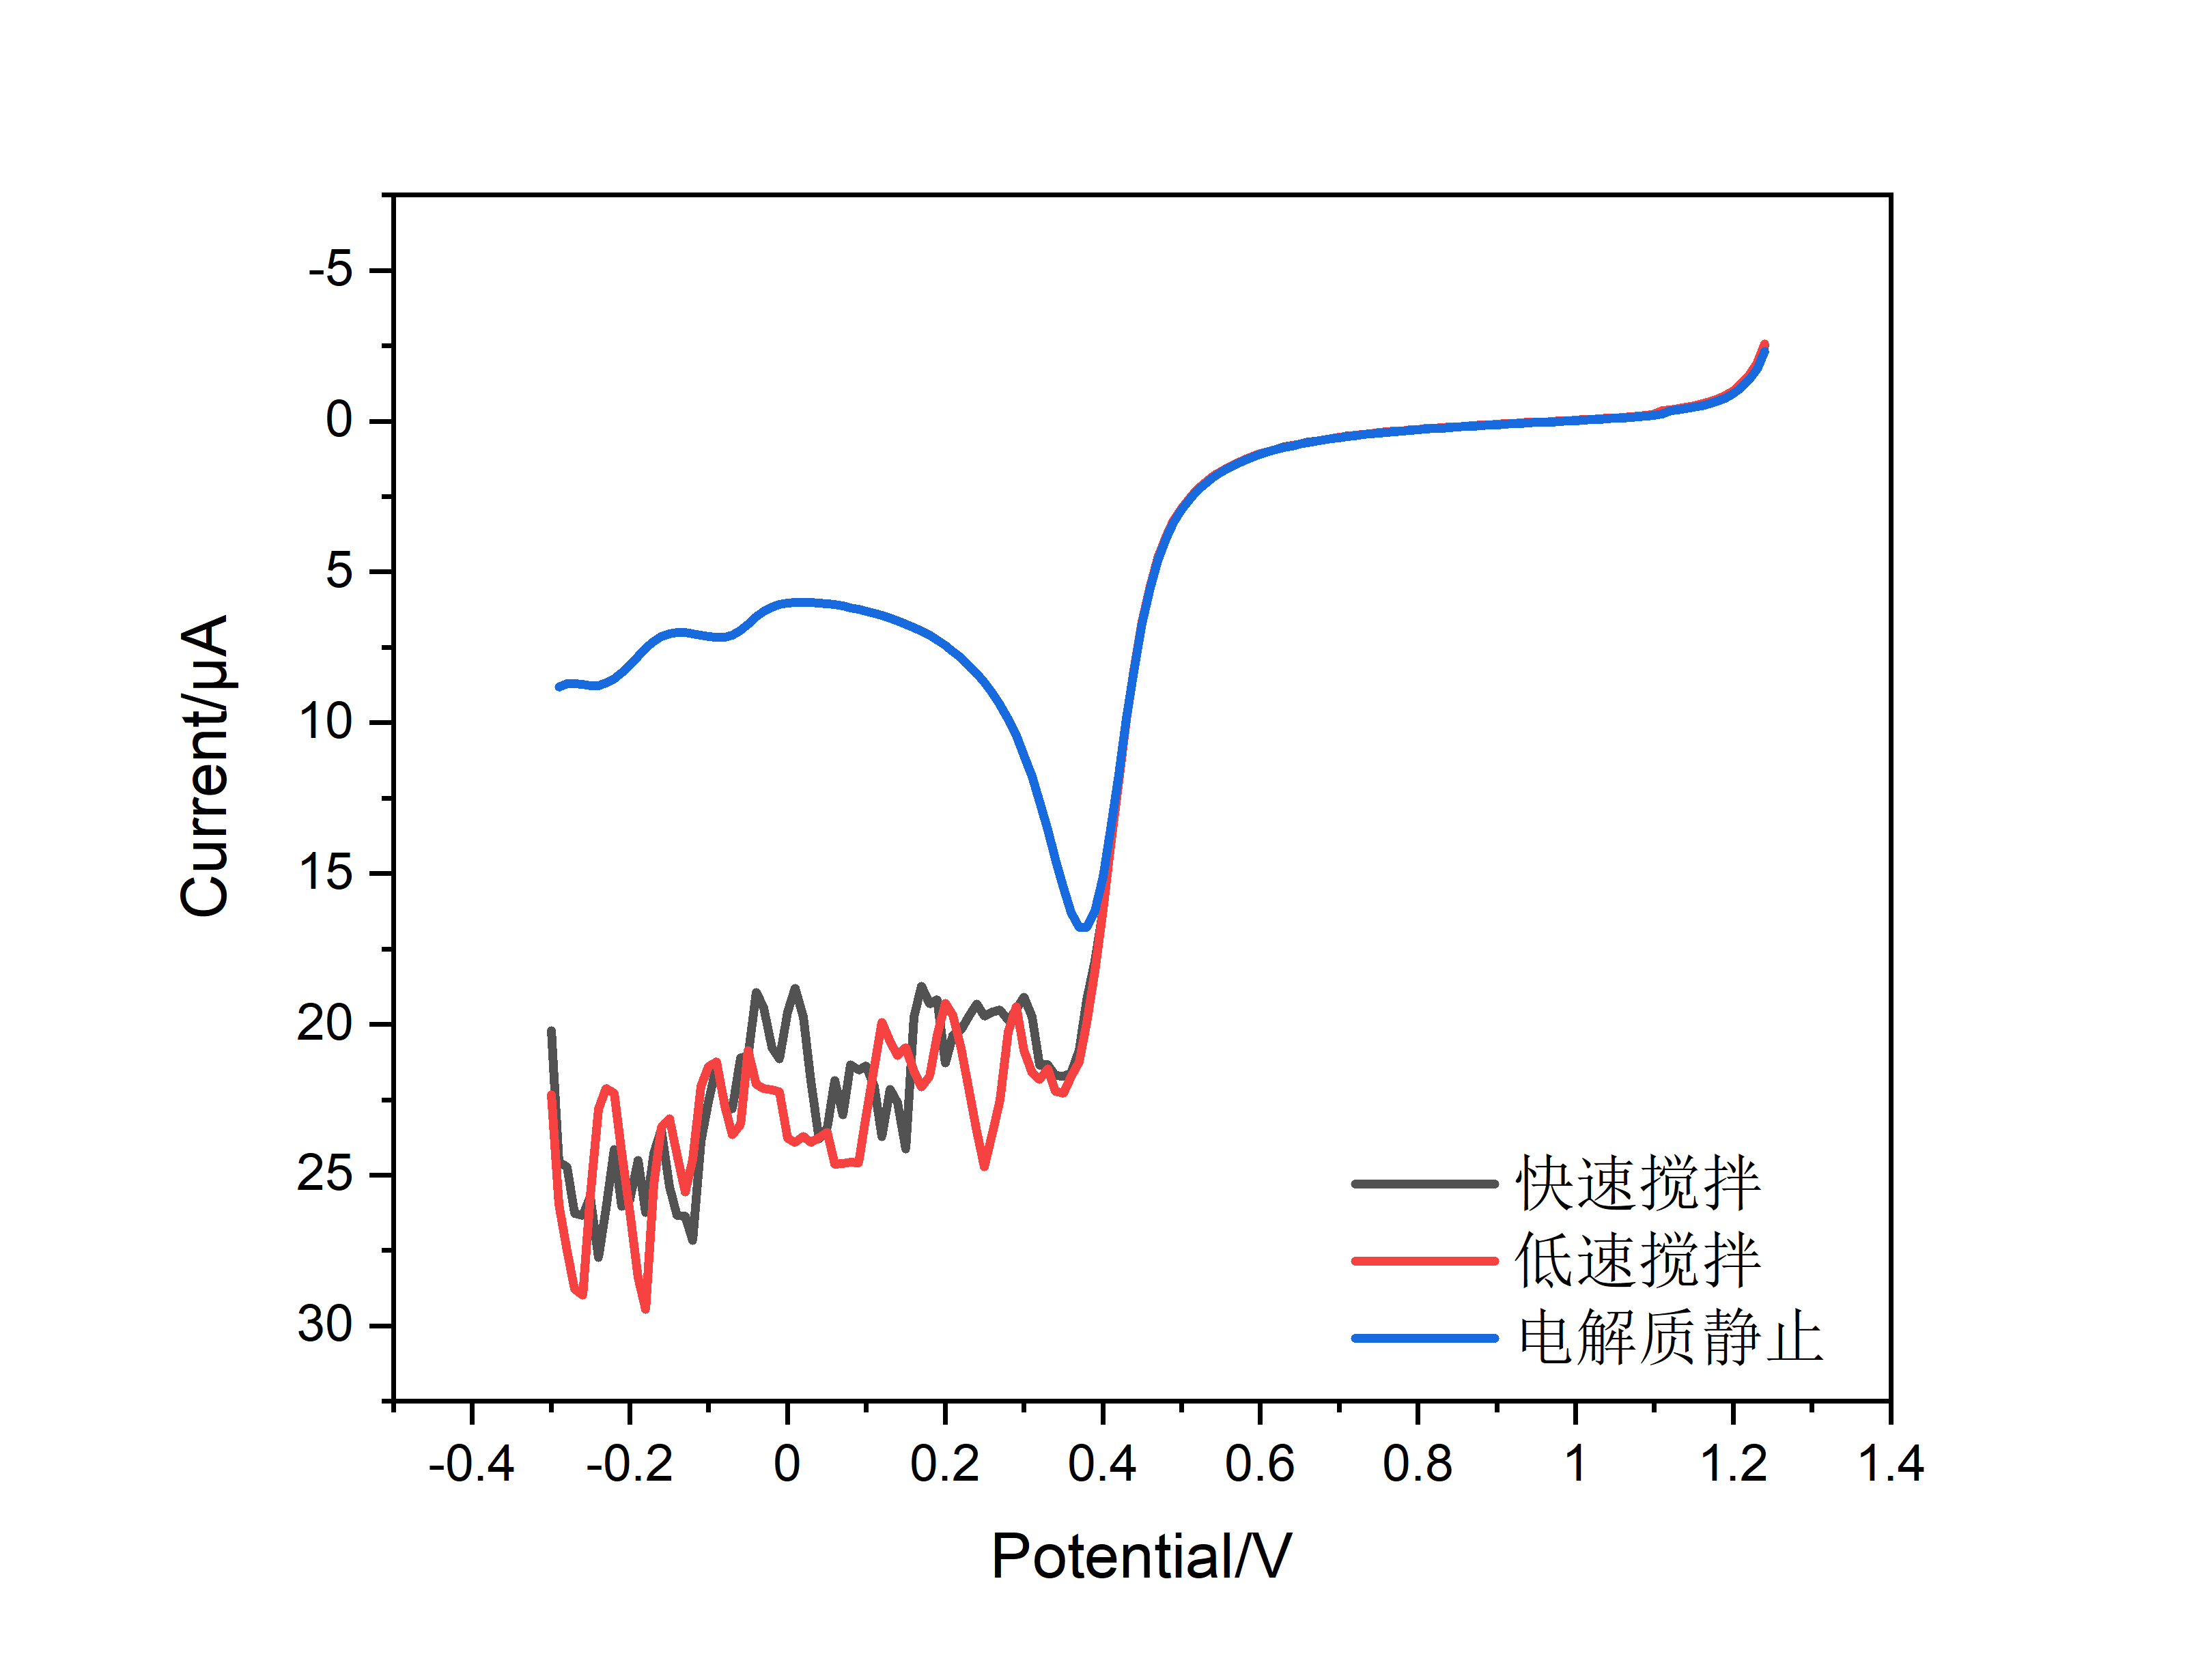
\includegraphics[width = .70\textwidth]{image/Graph2.png}
    \caption{不同搅拌速度下$\rm O_2$饱和的 0.05 M 硫酸水溶液中的 CV 曲线还原部分}\label{5}
\end{figure}

由图 \ref{5} 可以看出,当电势大于起始还原电位时,三条曲线几乎重合。此时决速步为电极反应,传质速率对
电流值的影响小,因此不同搅拌速度对结果的影响就也小。当电势小于起始还原电位时,搅拌+通氧气的高速搅拌组与通氧气的低速搅拌组相似,
而无搅拌的电解质静止组在电势较低时电流值较低。
在搅拌时,若过于剧烈, $\rm O_2$ 在电解质中分布不均,反应速率出现较大的波动,因此搅拌+通氧气组与通氧气组波动较大。
同时曲线也反应出,搅拌越快,传质越快使得反应速率升高,还原电流升高。

\begin{figure}[htbp]
    \centering
    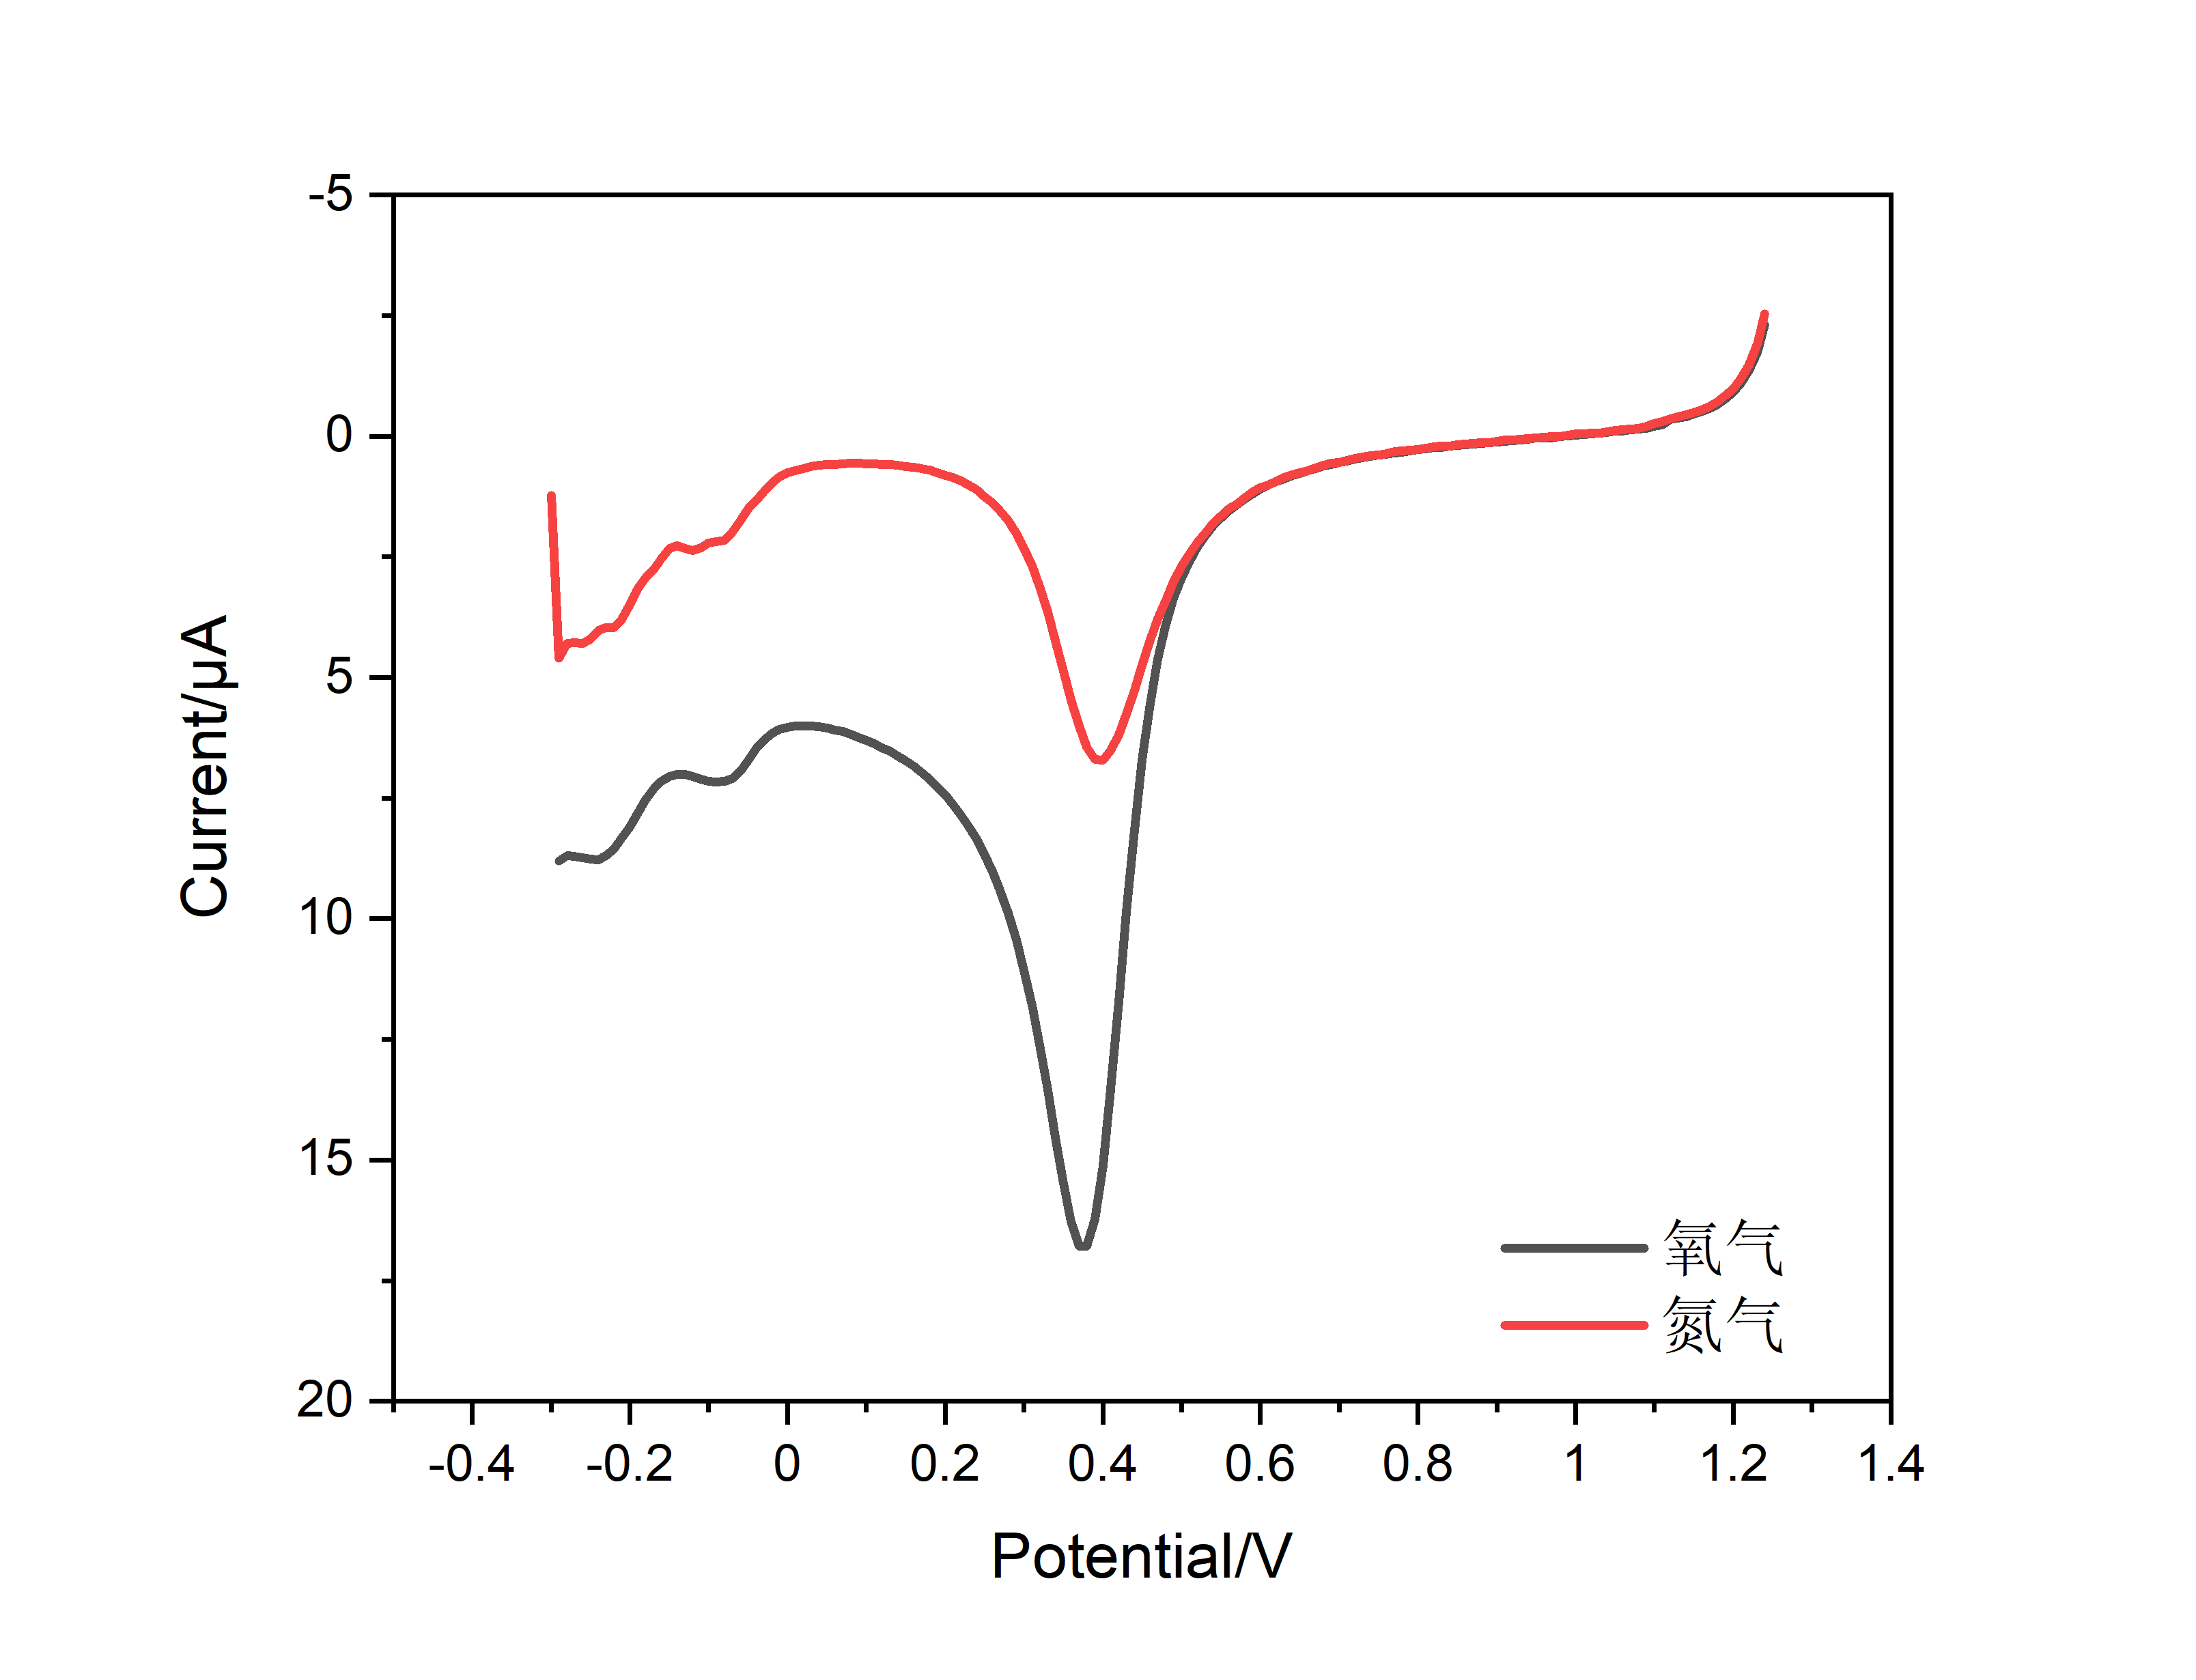
\includegraphics[width = .70\textwidth]{image/Graph9.png}
    \caption{$\rm O_2$ 与 $\rm N_2$ 饱和的硫酸溶液中铂电极的 CV 曲线还原支的叠加}\label{6}
\end{figure}

\begin{figure}[htbp]
    \centering
    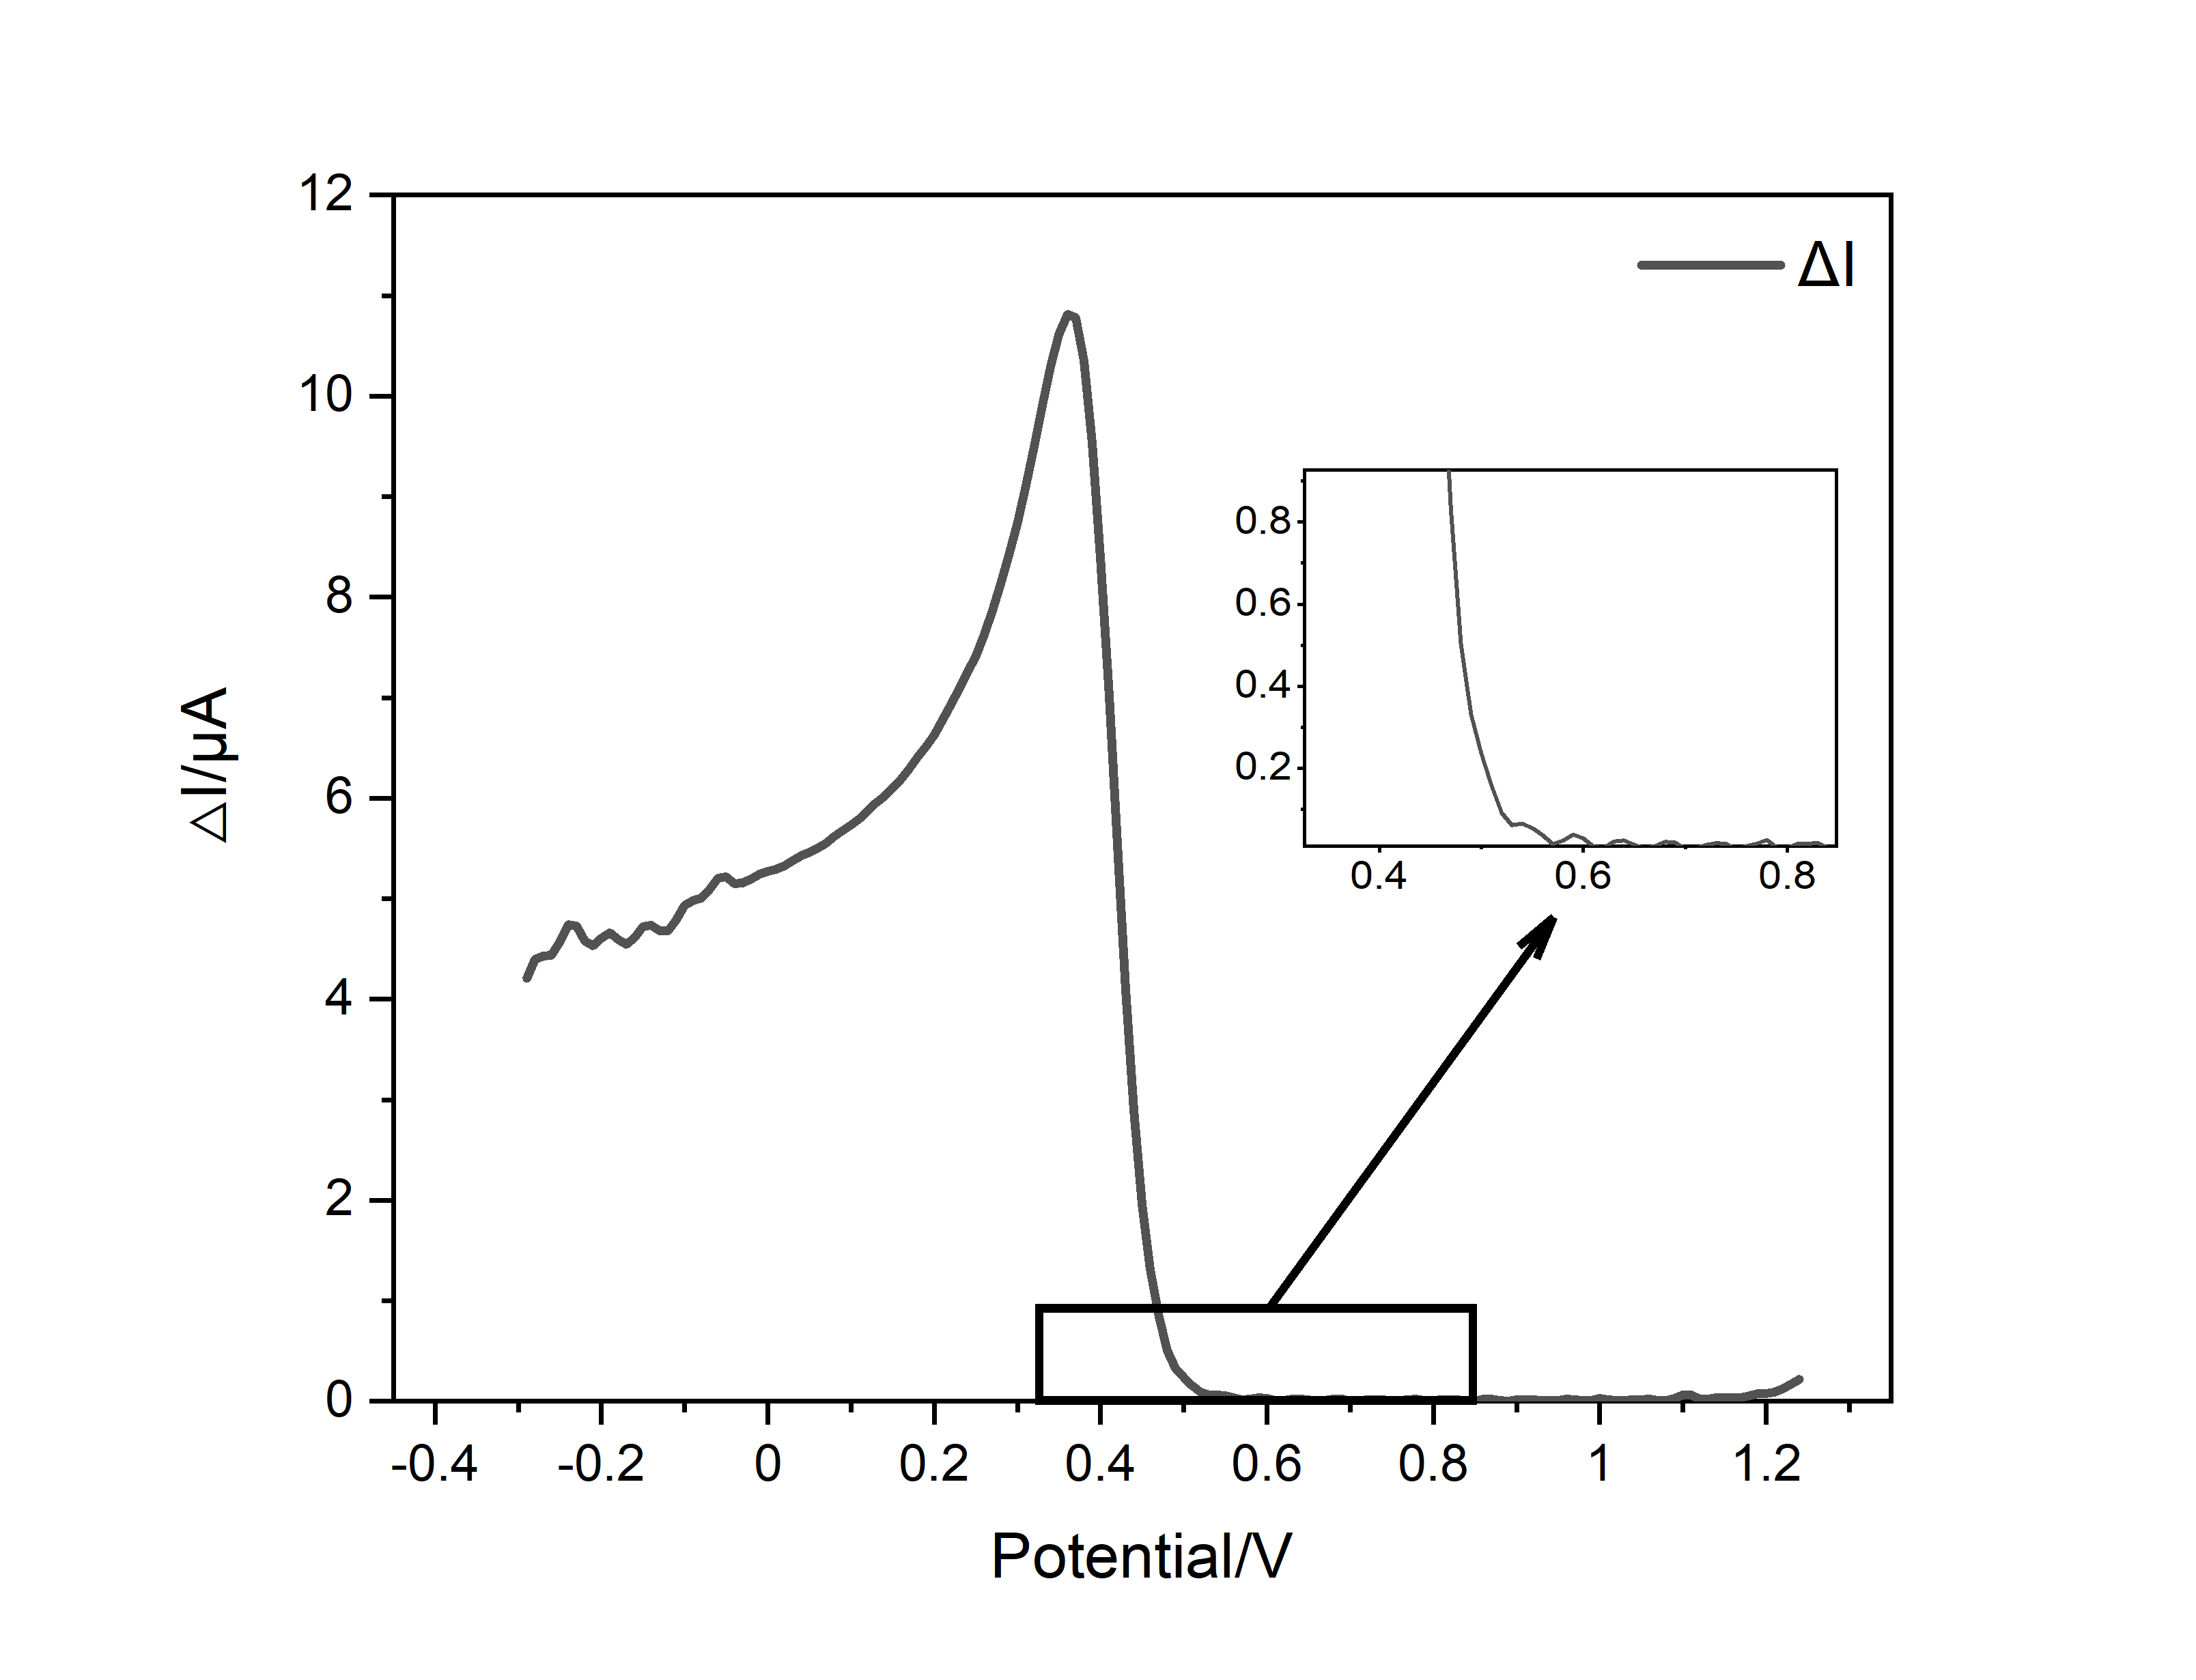
\includegraphics[width = .70\textwidth]{image/Graph10.png}
    \caption{$\rm O_2$ 与 $\rm N_2$ 饱和的硫酸溶液中铂电极的 CV 曲线还原支电流差}\label{7}
\end{figure}

在同条件下,使用 0.01 $\rm V \cdot s^{-1}$ 的扫描速度测定 LSV 曲线,如图 \ref{8} 所示。
可以看出,可以得到与 CV 相同的结论,但是由于扫速较慢,得到起始还原电位为 0.430 V,相比于 CV 曲线较低。


\begin{figure}[htbp]
    \centering
    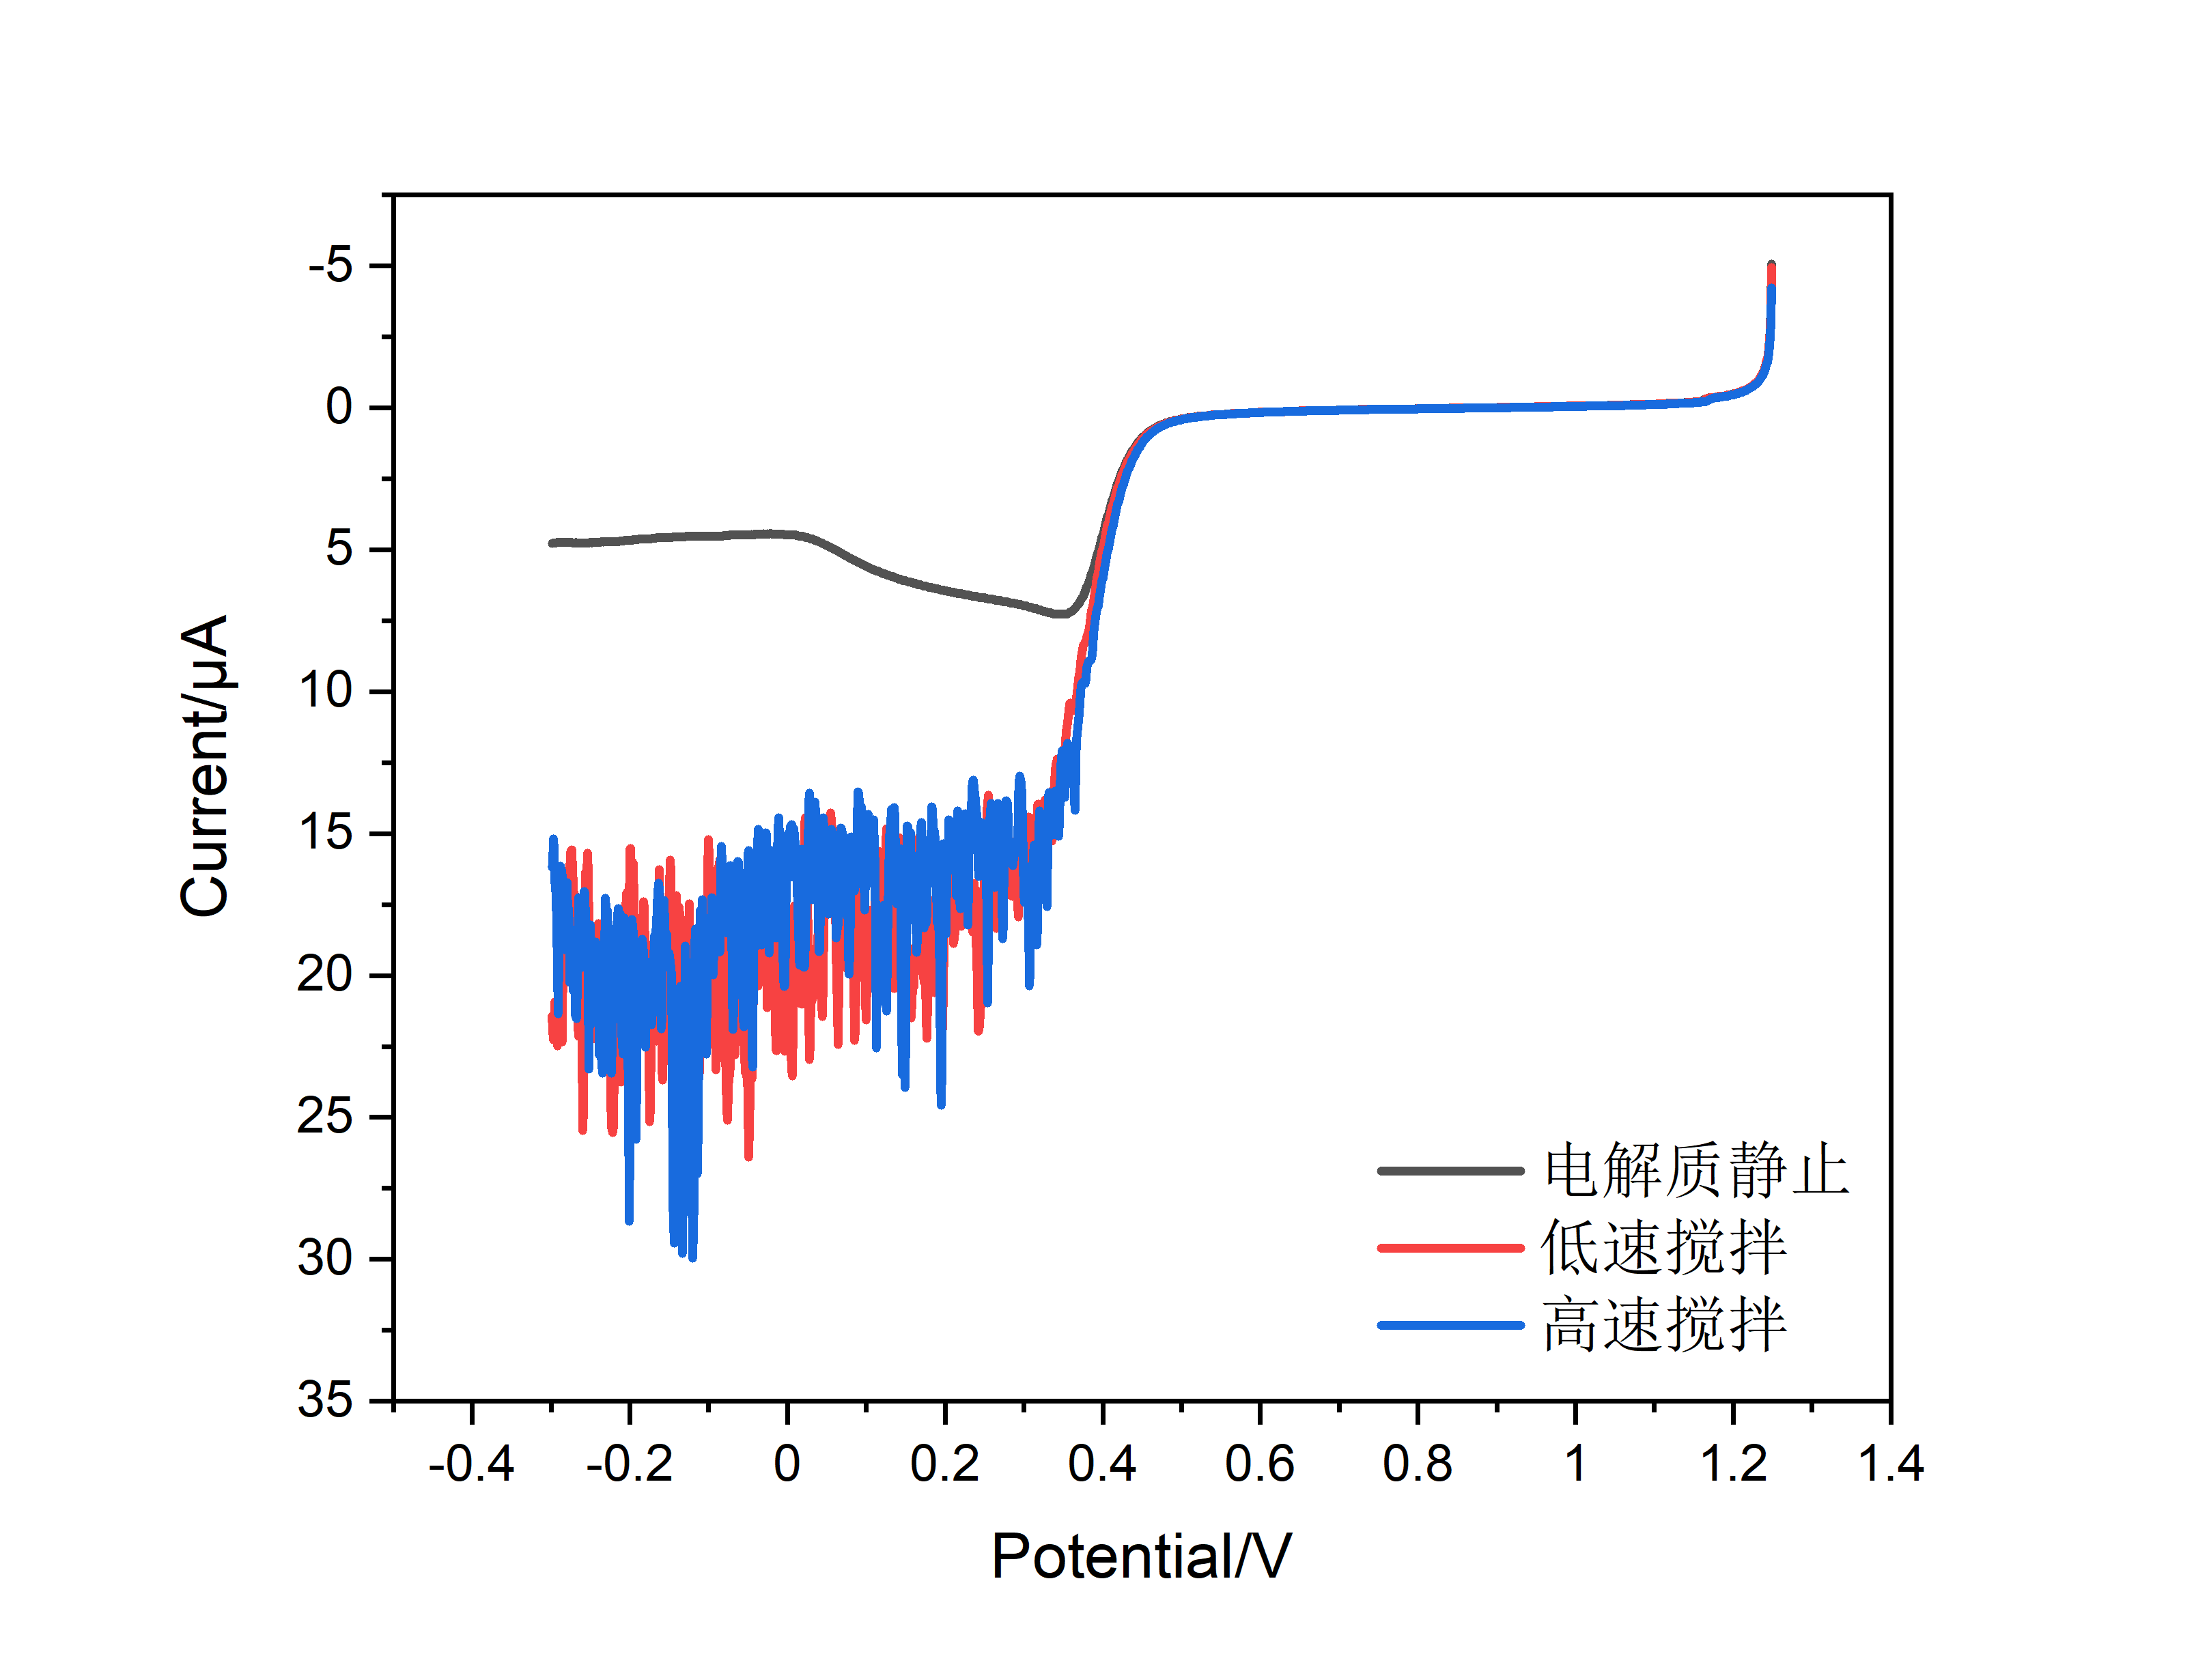
\includegraphics[width = .70\textwidth]{image/Graph1.png}
    \caption{不同搅拌速度下 $\rm O_2$ 饱和的 0.05 M 硫酸水溶液中的 LSV 曲线}\label{8}
\end{figure}

\begin{figure}[htbp]
    \centering
    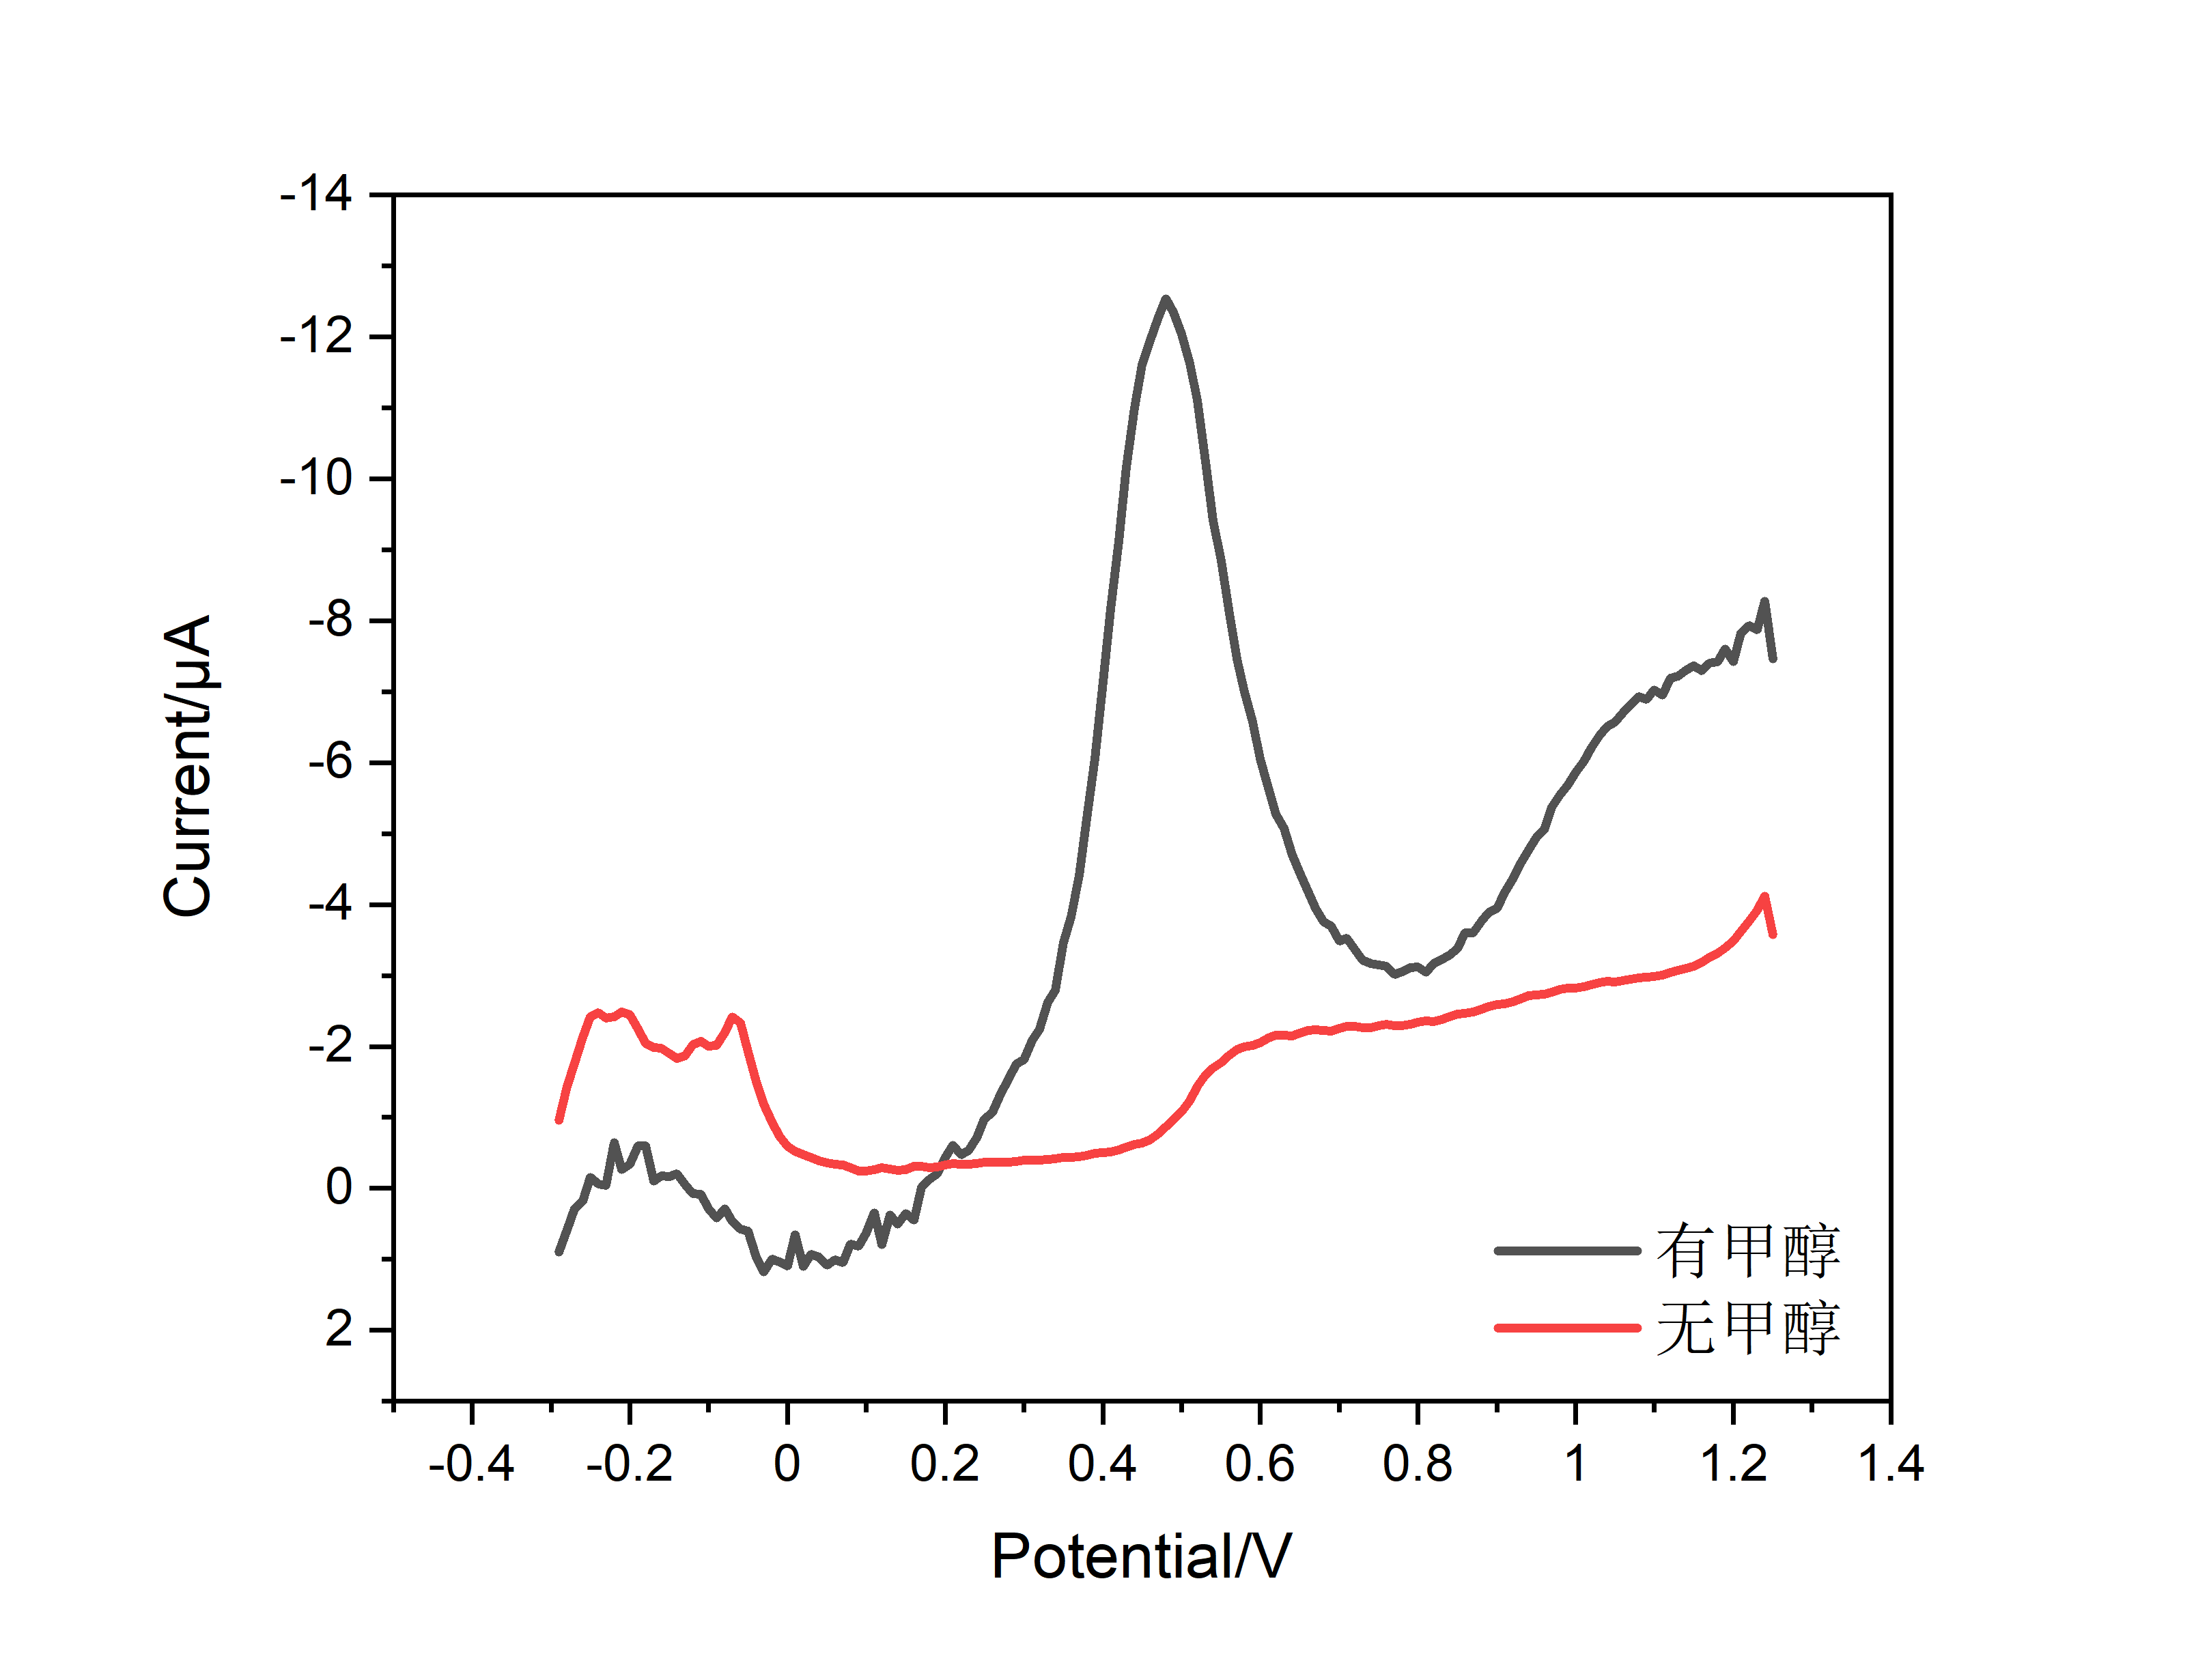
\includegraphics[width = .70\textwidth]{image/Graph4.png}
    \caption{有无甲醇的氮气下饱和硫酸溶液中铂电极的 CV 曲线}\label{9}
\end{figure}

\newpage

\subsection{测定甲醇水溶液的 CV 曲线}

在氮气饱和下,测量 0.1 mol/L 硫酸和 0.1 mol/L 甲醇水溶液等体积混合溶液的 CV 曲线,扫速为 0.1 V/s,取 Segment 7 作图如图 \ref{9} 
所示。由图可得,起始氧化电位为 0.210 V


\subsection{绘制 DMFC 电池的 U-P 曲线}

首先,需要确定DMFS的工作范围,DMFC 正常工作时,$\rm O_2$ 的还原电位应当高于 MeOH 的氧化电位。
因此,叠加扫速为 0.1 V/s 去除空白的甲醇硫酸溶液中 CV 曲线与 $\rm O_2$ 的饱和硫酸溶液
中 CV 曲线的相反数。取两者的重叠部分即为工作范围。工作范围为0.190 - 0.990 V,工作电流为 0 - 9.861 $\rm \mu A$,二者的交点处电压为 0.430 V。


\begin{figure}[htbp]
    \centering
    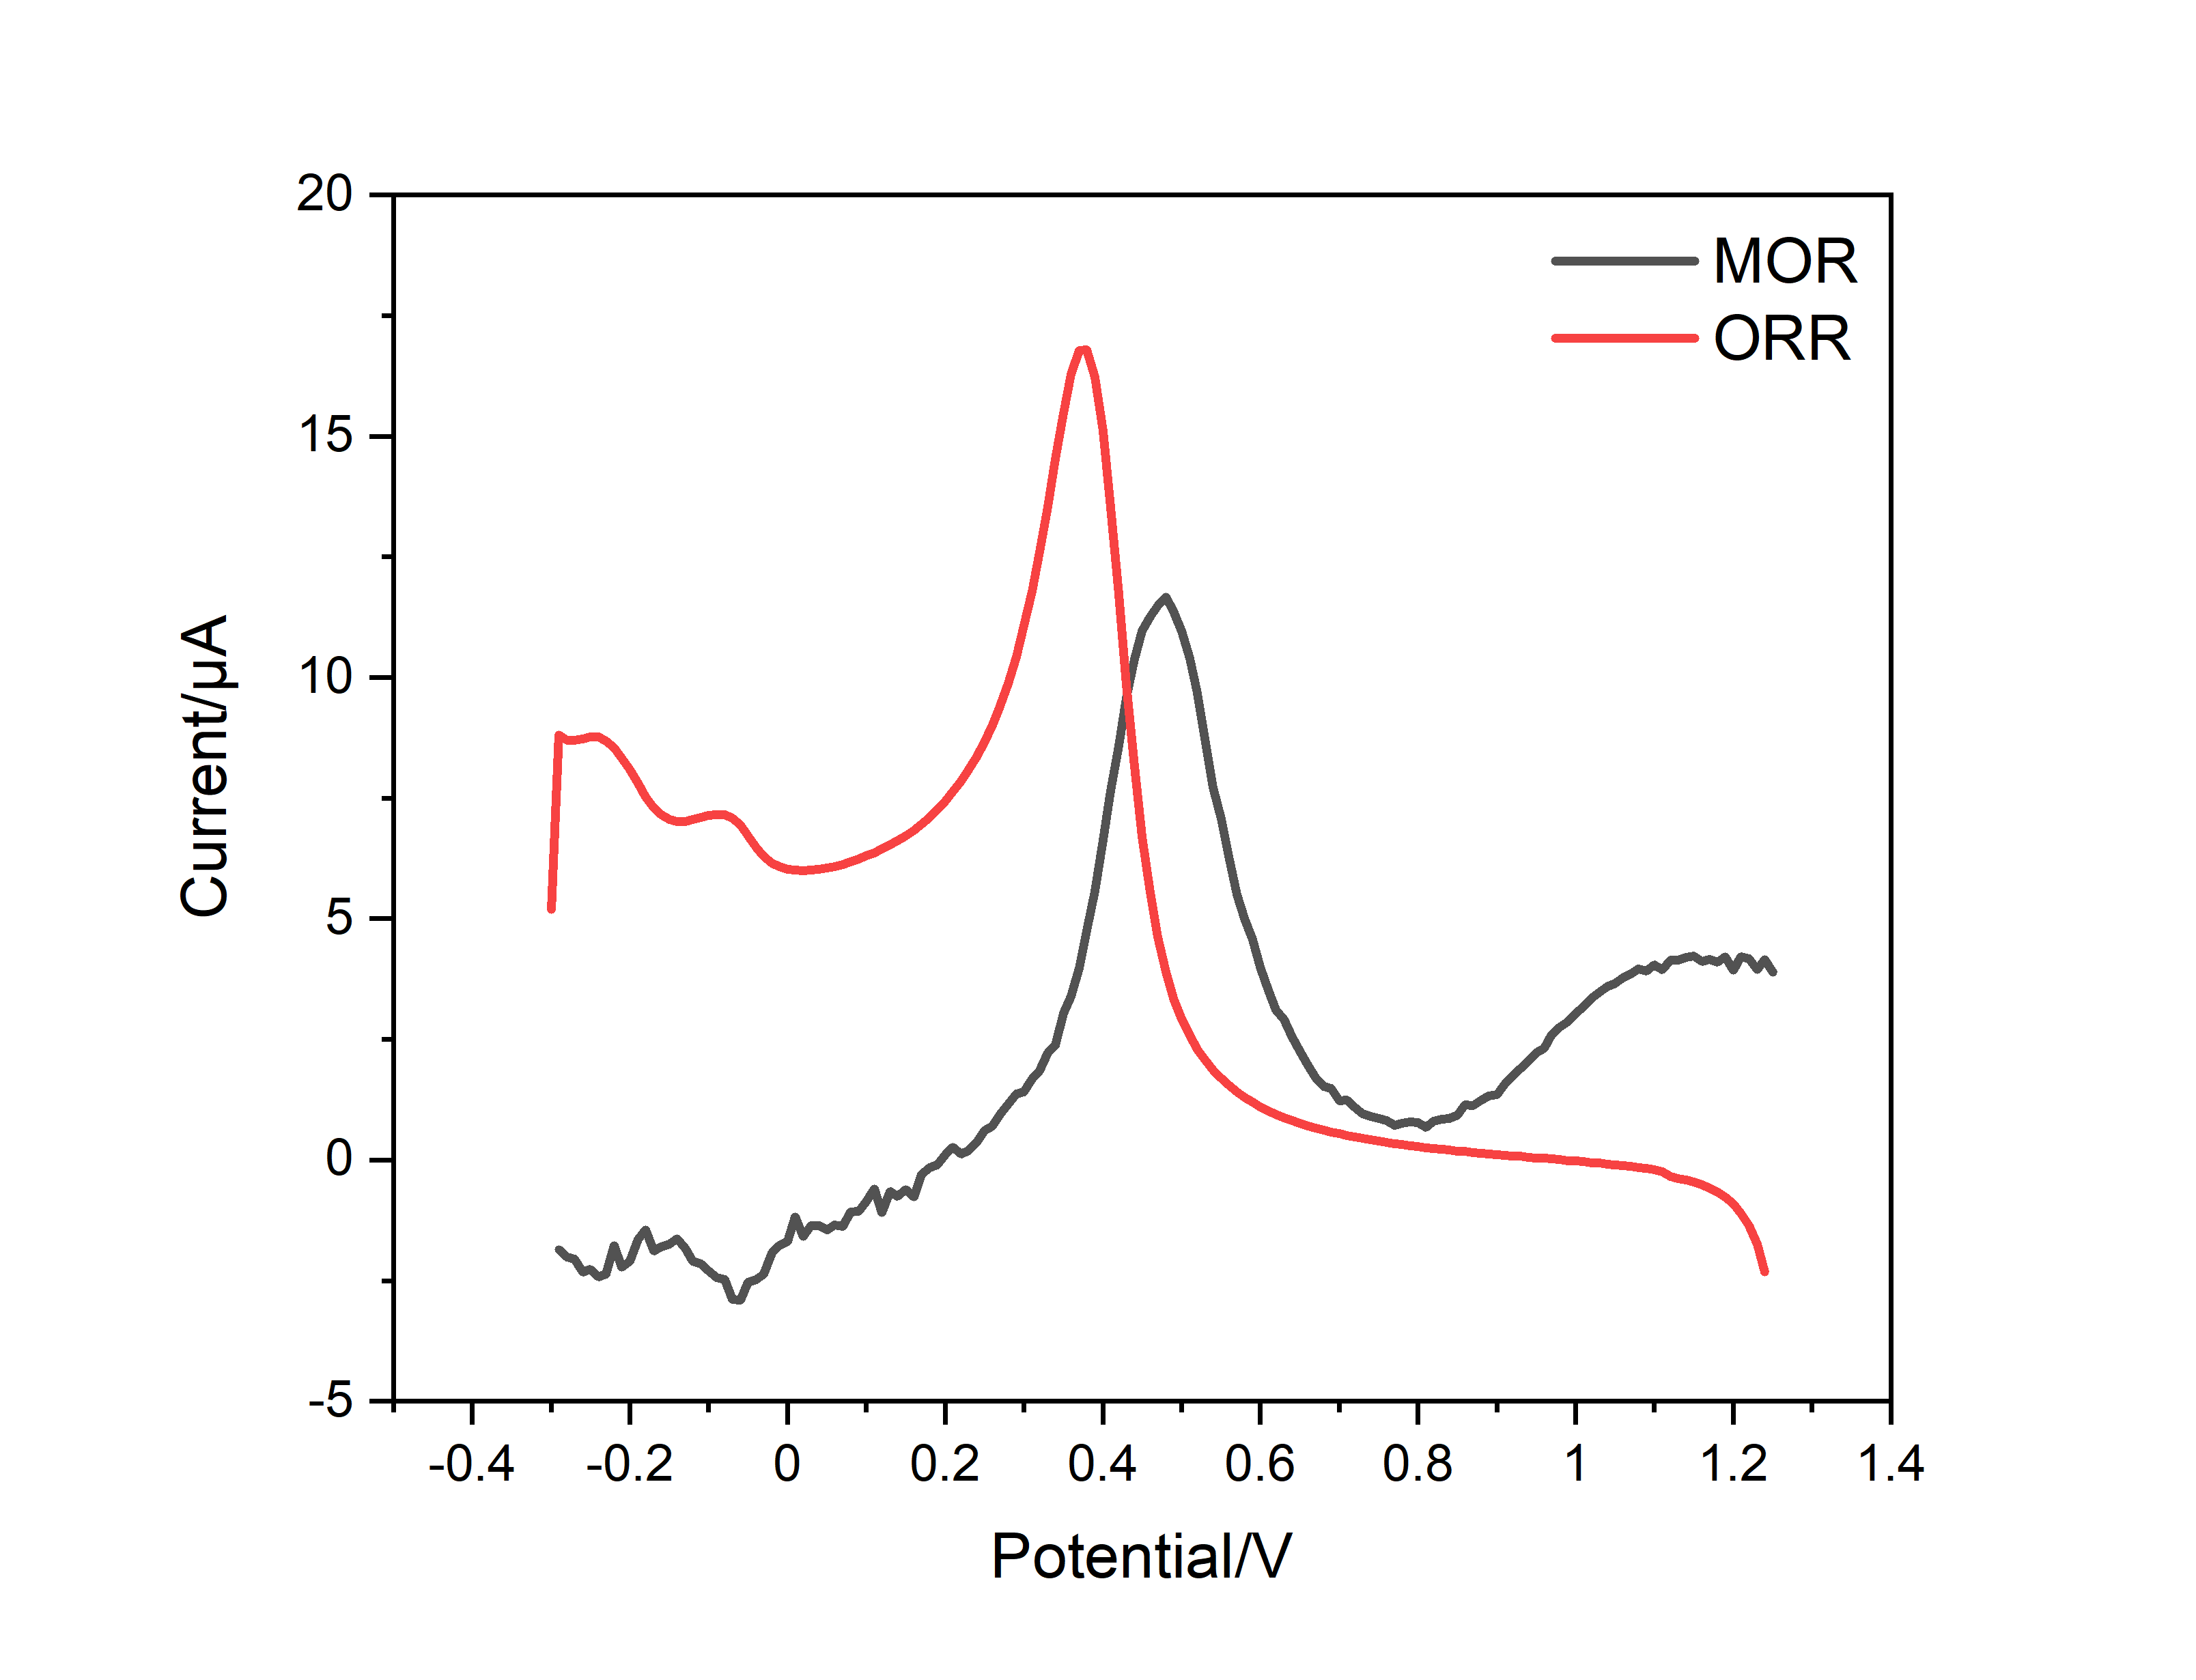
\includegraphics[width = .70\textwidth]{image/Graph8.png}
    \caption{确定 DMFC 工作范围}\label{10}
\end{figure}

对工作范围内的两种曲线进行作图,得到 DMFC 极化曲线,如图 \ref{11} 所示。

\begin{figure}[htbp]
    \centering
    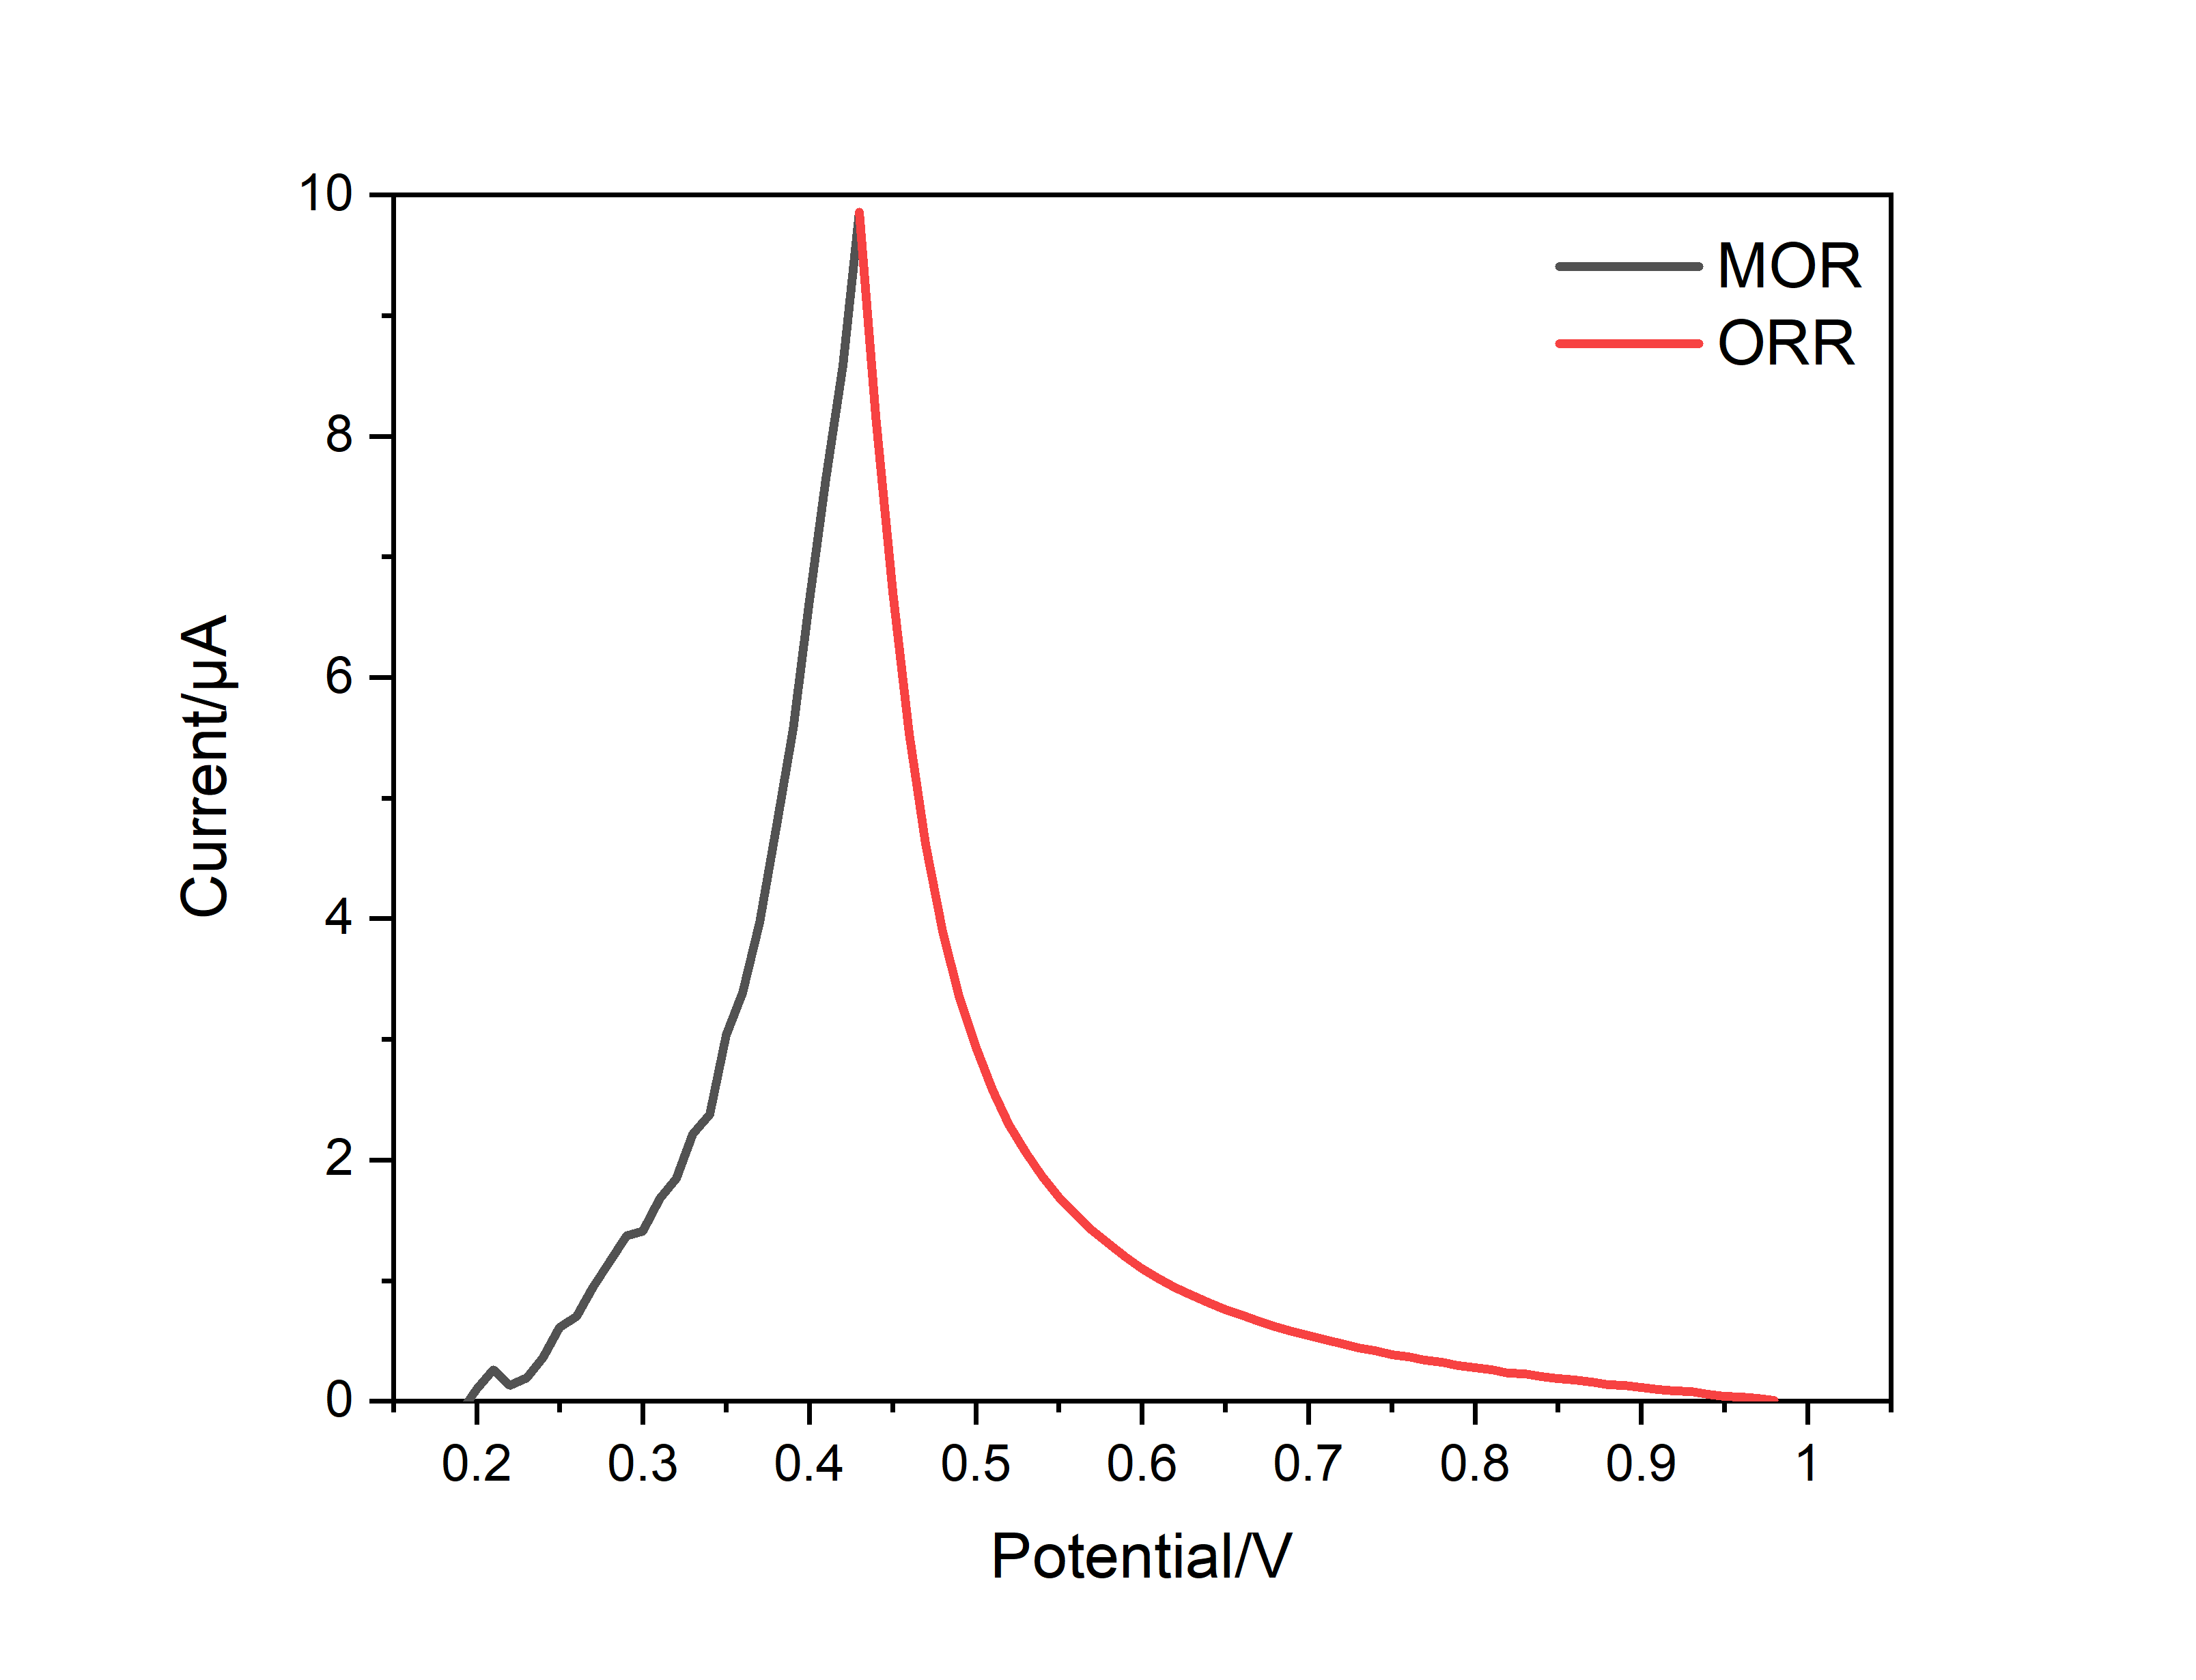
\includegraphics[width = .70\textwidth]{image/Graph12.png}
    \caption{DMFC 极化曲线}\label{11}
\end{figure}

对曲线上取点,由公式
$$
P = UI
$$

得到可得输出电压-输出功率曲线如下图 \ref{12} 所示。输出功率随着电压的增大先增大后减小,但是图像右侧有些许抖动,应该为 MOR 的 CV 曲线不太平滑导致的。由图中可以得到最大功率时,电压为 0.35 V,
功率为 0.243 $\rm \mu W$。

\begin{figure}[htbp]
    \centering
    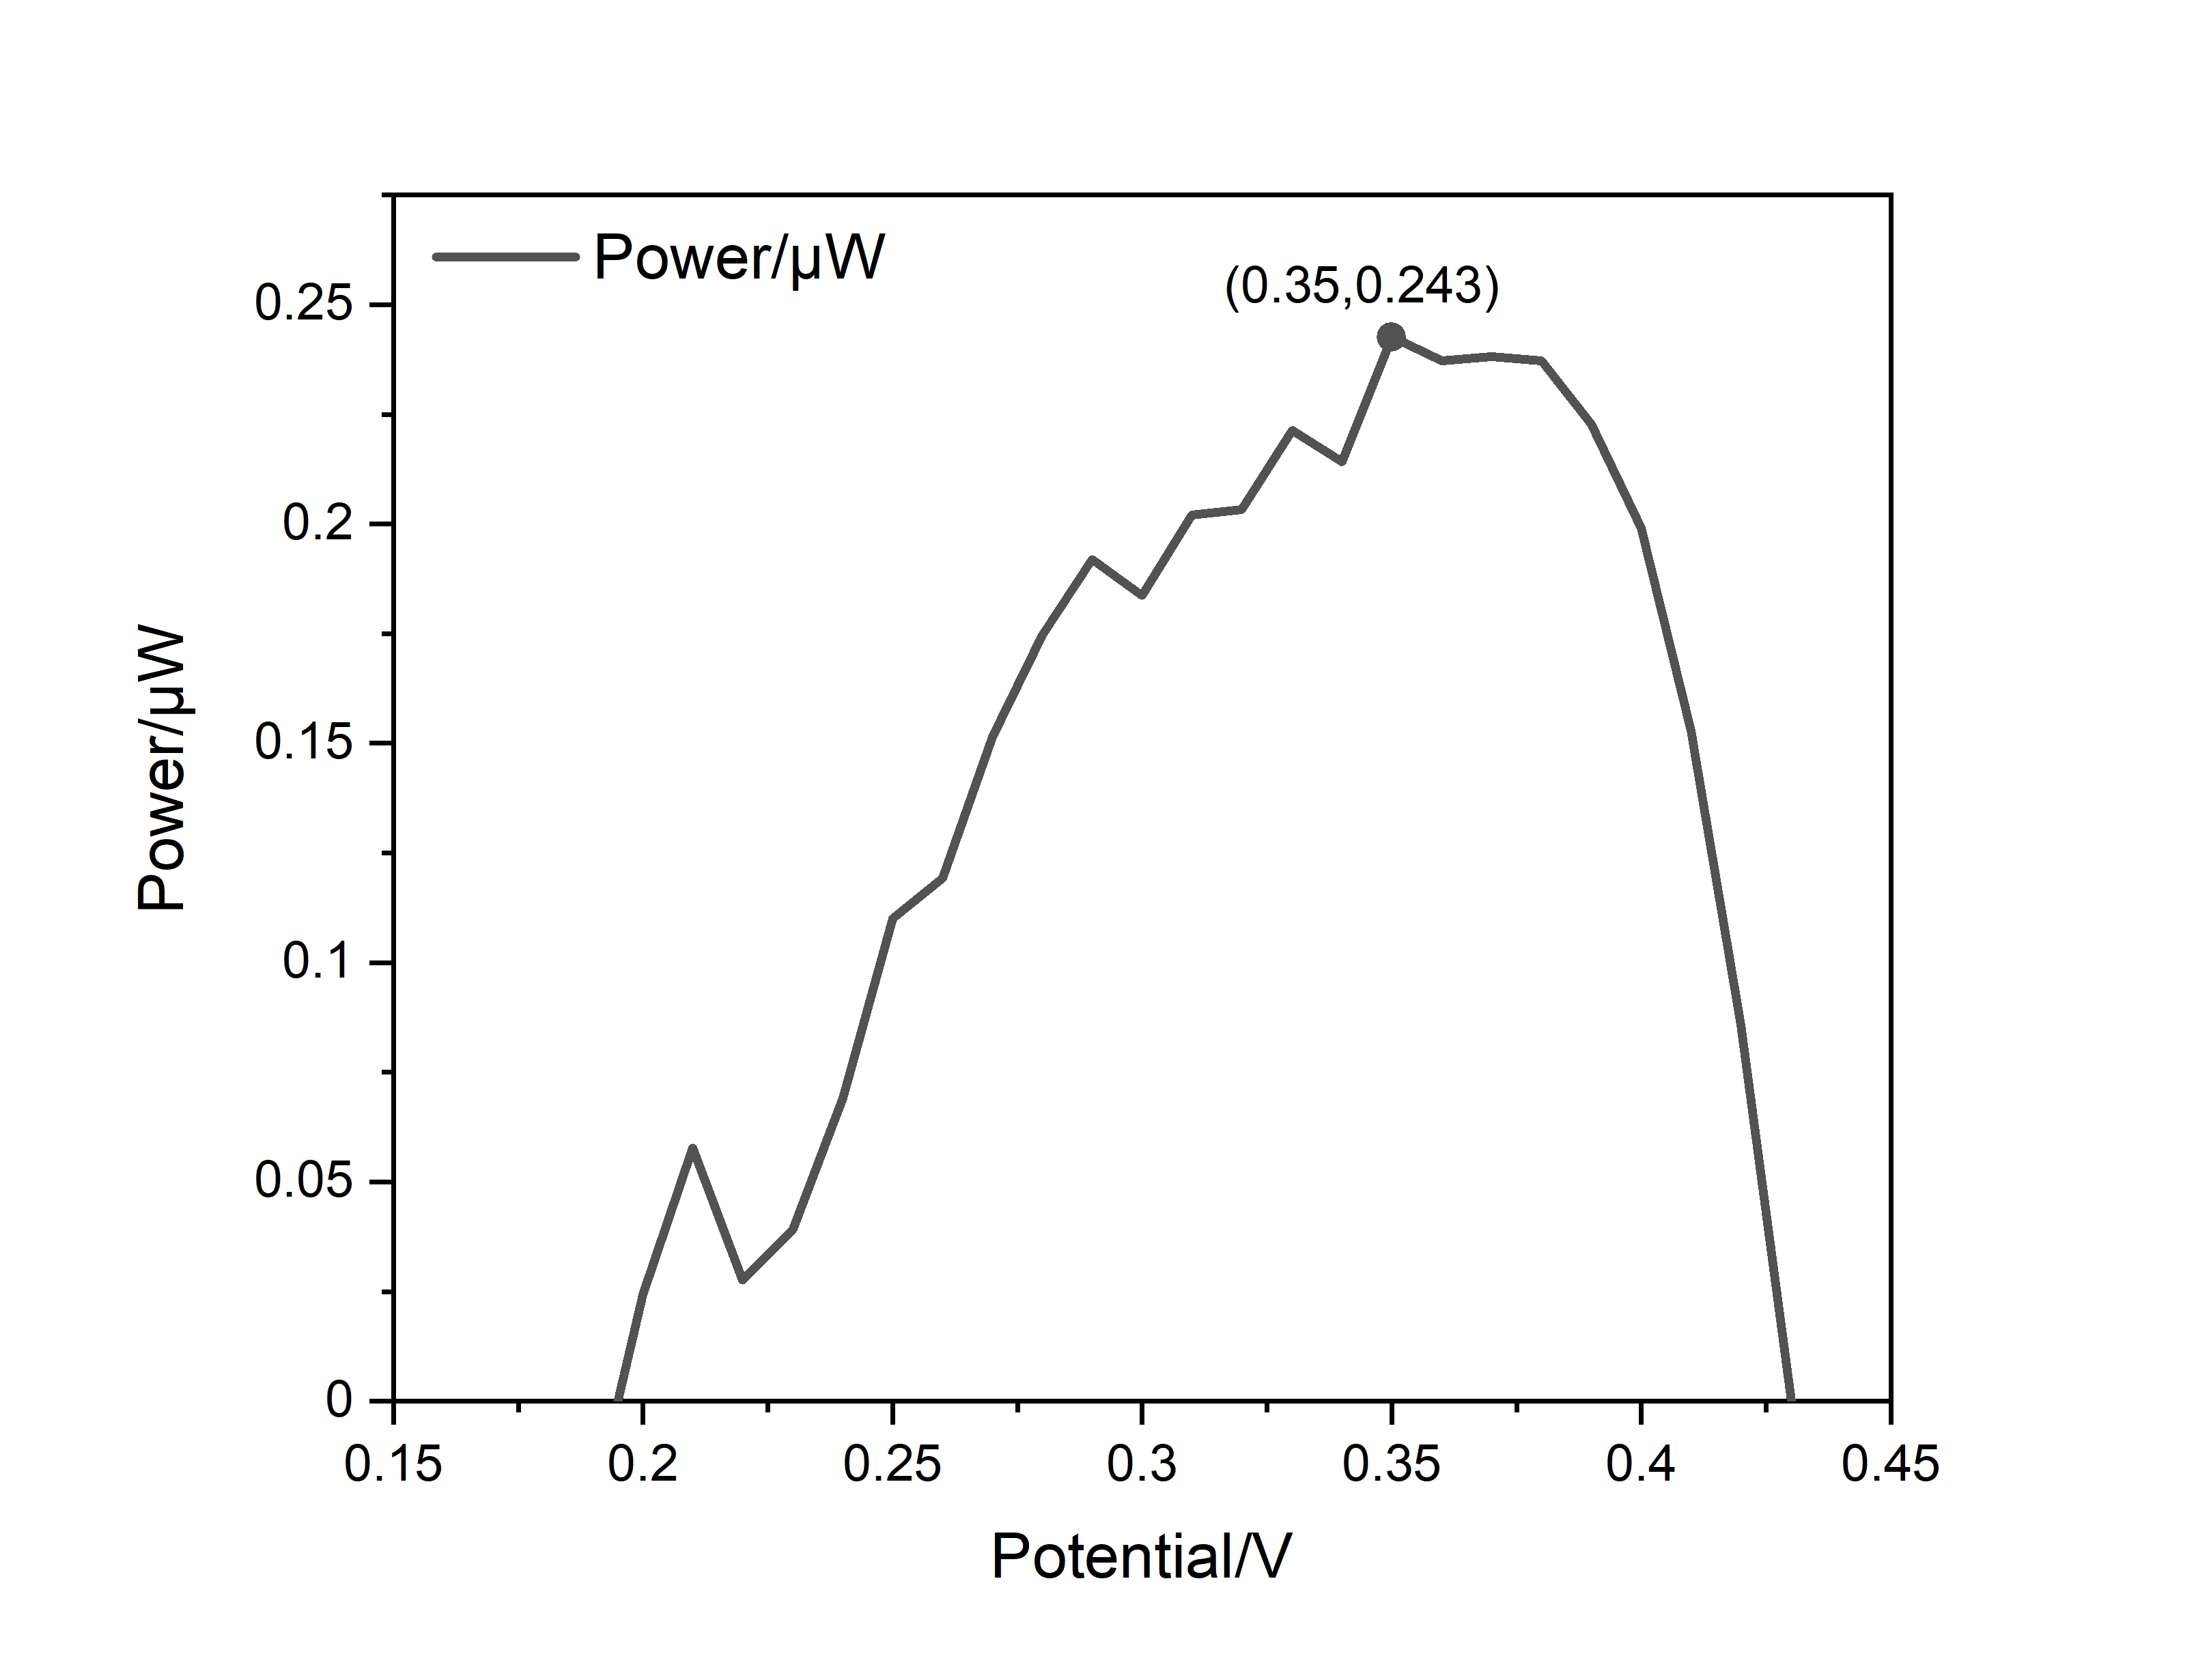
\includegraphics[width = .70\textwidth]{image/Graph14.png}
    \caption{DMFC 电池的 P-U 曲线}\label{12}
\end{figure}


\newpage

\section{实验结果与讨论}

\subsection{结论}

    本次实验采用循环伏安法与线性扫描伏安法,对氧气电化学还原反应 (ORR) 与甲醇电化学氧化反应 (MOR) 
进行测量。得到 ORR 在扫速为 0.1 V/s 下起始还原电位为 0.590 V,MOR 在扫速为 0.1 V/s 下起始氧化电位为 0.210 V
。
通过实验数据分析,我们可以观察得到扫描速度与搅拌速率对 CV 曲线的影响。扫描速率越快
电流峰值时的电压值近乎不变,而电流峰值升高;搅拌速率升高,传质速率升高,反应速率加快
因此还原电流升高。同时由于浓度分布不均,还原电流会出现振荡现象。

根据实验数据还可以计算出铂电极的电化学活性面积为 ESA = 2.39 $\rm mm^2$。
通过 ORR 与 MOR 的 CV 曲线,利用取点法可以计算得到甲醇直接燃料电池的极化曲线与输出
功率-输出电压曲线。在甲醇直接燃料电池最大功率时,电压为 0.35 V,
功率为 0.243 $\rm \mu W$。


\nocite{*}
\bibliography{reference}
\end{document}
